% ============================================================
%  第三卷 第十二章 对称性理论（§91–§99 + 习题）
%  底本：高教社中文版第6版（严肃 译，喀兴林 校）
%  OCR 底稿 full_merged.md 行 13038–13937
%  插图：图32–图40（figures/fig32.pdf–fig40.pdf）
%
%  已修正的 OCR/原书错误（均对照 原书转换/pages/p-340…p-373.png 核实）：
%   [§91] 行13106–13108 乱句按原书 p329 重建（“现在来指出，转角为 π 转轴
%         （图33中的 Oa 和 Ob）相交成角 φ 的两个旋转……Oa′ 和 Oa 的夹角为
%         2φ. 用同样的方法还可证明……相反的方向.”，OCR “变快的结果仍寺
%         十一个庭转”等）；Iσ_h、IC_2=σ_h 的下标 OCR 误作 \hbar；
%         σ 的下标 ν→v（全章统一，v=竖直面、h=水平面）；行13046 把这个
%         操作重复进行两次（OCR 衍入记号 C_n）；(91.6) σ_vσ_v′ 按 p328
%         恢复（OCR “\sigma,\sigma′”）；“从 σ_v′ 面到 σ_v 面”按 p329 恢复.
%   [§92] 满足 AA^{-1}=E（OCR 衍 A^{-1}）；H_aG_1=H_b、G_1=H_a^{-1}H_b
%         （OCR H_6、G_ι）；B=P^{-1}AP、C=Q^{-1}BQ 按 p331 恢复；
%         (CAC^{-1})^n=CA^nC^{-1}=E（OCR 末项作 1，按 p332 为 E）；
%         共轭类一段“共轭元类（或简称类）”按 p331 补全.
%   [§92–§99] 直积记号 OCR 之 \circledast、\textcircled{×}、(×) 一律按原书
%         排 \otimes；群名黑斜体照原书排 \boldsymbol（p330 脚注②体例），
%         群元/算符/矩阵元用斜体.
%   [§93] 行13264 显示公式 σ_dS_{2n}^{2k+1}σ_d=σ_hC_{2n}^{-2k-1}=S_{2n}^{-2k-1}
%         系脚注①文字窜入正文，按 p336 从正文删除；(S_{4p+2})^{2p+1}
%         =C_2σ_h=I（原书小写 c_2 排印误，按上下文改 C_2）；
%         S_{4p+2}=C_{2p+1}⊗C_i、也记作 C_{2p+1,i}（OCR S_{a_{p+2}} 乱）；
%         C_{1h} 又记作 C_s（OCR 乱码）；群名 C_{2p,v}、C_{nv}、D_{nh}、
%         D_{2p,h}、D_{nd}、D_{2p,d}、D_{2p+1,d} 等按 p333–336 恢复；
%         IX 节 “6 个 S_4 和 S_4^3 旋转-反射变换”（OCR S_\varphi）；
%         “加进一个水平对称面通过 n 个二阶轴”照原书 p335.
%   [§94] 开篇 ψ_1/ψ 混排按 p338 恢复（设 ψ_1 为……坐标单值函数；对于
%         某种 ψ_1 讲来）；(94.2) ψ_i^·→ψ_i^*；求和号 ∑_σ→∑_G；
%         (94.9) δ_{km}（OCR \delta_{\boldsymbol{k}m}）；(94.11) g_C、
%         巡标 C；r^2 个量 f_{αC}=\sqrt{g_C/g}\,χ^{(α)}(C)（OCR 下标 c）；
%         对第二个下标的正交式 ∑_α f_{αC}f_{αC′}^*=δ_{CC′} 按 p341 补全
%         （OCR 漏 f_{αC}f^* 因子）；(94.12) δ_{CC′}（OCR δ_{CC^*}）；
%         (94.13) 首和号原书印作 ∑_C，按上下文改 ∑_G（原书排印误）；
%         “对于一个阿贝尔群（此时 r=g）”（OCR \mathfrak{D}_ε 乱码）；
%         (94.18) 后 Ĝψ_i^{(α)}=∑_l G_{li}^{(α)}ψ_l^{(α)} 按 p342 恢复
%         （OCR ∑_e、ψ_l 误作 ψ_i）；(94.19) 第二式求和号 ∑_α→∑_G；
%         “么正算符”“幺正矩阵”照原书 p339 混用排.
%   [§95] ε=e^{2πi/3}（OCR 作 e^{2πi√3}）；√[g]{1} 因子；
%         表7 全部按原书 p346–347 重排为 tabular（OCR 的 HTML 表彻底
%         错乱不可用），逐格核对：C_i/C_2/C_s 块、C_3 块（E;x±iy 两行）、
%         C_2h/C_2v/V=D_2 块、C_3v/D_3 与 C_4/S_4 块（S_4 列 B;z 与
%         E;x±iy 加右花括号照原书）、C_6 块（E_1、E_2;x±iy 两对复共轭行，
%         E_1 行 χ(C_6)=ω^2、E_2;x±iy 行 χ(C_6)=ω，照原书 p346）、
%         C_4v/D_4/D_2d 块、D_6/C_6v/D_3h 块、T 块（E 两行 ε/ε²）、
%         O/T_d 块；D_3d 特征标表按 p348 重排；表7 首块第二行数值原书
%         上下两行均印作 (1, −1)，上行（A_g、A;z、A′;x,y）按物理与
%         p346 页面核为排印误，改正为 (1, 1).
%   [§96] F_2（T_d）、C_3v、C_2v 三个特征标行按 p349–350 重排.
%   [§97] 证明中 g∫ψ_i^{(α)}dq=∑_k∫ψ_k^{(α)}∑_G G_{ki}^{(α)}dq（OCR 中间
%         ψ_k 误作 ψ_i，按 p350）；习题 1 “对称 O”（OCR 对称0）；
%         习题公式 (1)–(4) 按原书右花括号+编号排，用节内 equation 计数器
%         重置实现（仿卷3 ch05 体例）；μ_z 选择定则按 p352.
%   [§98] 首段 C_∞ 群（OCR c_∞，且勿与 C_∞v 混，按 p353 “两维旋转群”）；
%         D_∞h=C_∞v⊗C_i（OCR 漏 v）；(98.1)(98.2) 指标 G_{ik}G_{lm}^* 按
%         p354；dτ_G=sin β dα dβ dγ、∫dτ_G=8π²；χ^{(J)}(φ) 未编号式与
%         (98.3) 按原书；“欧拉角”“欧勒角”照原书混用；(98.5) C_∞v 特征标
%         表按 p356 排为编号公式.
%   [§99] 反射可写成 σ_h=IC_2（OCR σ_k）；群 D′_n（OCR \delta_p′）；
%         绕二阶水平轴……e^{±2πik/n}（OCR 衍空格）；χ(C_2Q)=−χ(C_2)、
%         χ(C_2)=0 一句按 p358；a_1=e^{πi/3}、a_2=e^{−πi/3}；反对称积
%         {D^{(α)2}} 和对称积 [D^{(α)2}]（行13926 乱，按 p359）；
%         表8 全部按原书 p358–359 重排为 tabular，类配对 [C_n^k /
%         C_n^{2n-k}Q] 照原书（双群中 C_n^k∼C_n^{2n-k} 相共轭）；D′_2
%         类头第三列上行原书两行均印 C_2^{(z)}Q，上行按同类规则改
%         C_2^{(z)}；T′ 的 G′、O′ 的 E_1′/E_2′/G′ 各行逐格核对.
%   [§99 习题] J 表按 p360 恢复：0→A_1、1/2→E_1′、1→F_1、3/2→G′、
%         2→E+F_2、5/2→E_2′+G′、3→A_2+F_1+F_2（OCR “3/”缺 2）.
%   [全章] 圈码①②③共 36 处原样保留（脚注文本由脚注代理转录），一处
%         未丢；\mathrm{d} 收紧；函数名 \sin\cos 正体；半角标点按文体
%         约定改全角；OCR 的 \pmb/\boldsymbol 误标（群元 G、算符 Ĝ、
%         矩阵元 G_{ki} 等）按原书改回斜体.
%
%  脚注转录（脚注代理，2026-10-11，按 pages300 p341–p372 页面实况逐条
%  核录，共 36 处：\footnote 取代原圈码，footmisc[perpage] 按页自动圈码）：
%   - 页码分布：p341(1) p343(2) p347(1) p349(1) p350(1) p351(1) p352(2)
%     p353(1) p355(1) p357(1) p358(3) p360(1) p361(2) p362(3) p363(1)
%     p364(1) p365(1) p367(1) p368(3) p369(2) p370(3) p371(1) p372(2)；
%   - 公式类脚注：p349①（σ_d S_{2n}^{2k+1}σ_d=…=S_{2n}^{-2k-1} 显示式，
%     即排版期从行13264 正文删除的窜入内容，此处归位）、p357①
%     （{χ²}(G)=det 特征标式）、p358②③（ψ=e^{ikφ} 等）、p365①
%     （[D^{(α)2}] 含单位表示）、p369①（(98.2) 式积分权函数）、
%     p370③（S′_2≡C′_i、S′_6≡C′_{3i}）、p371①（χ(C_n^k)=(−1)^k）；
%   - p343① 为双段长脚注（置换群说明＋本章记号约定"加 ^ 号/黑斜体群名"
%     的出处），footnote 内以 \par 分段；
%   - p358③ 的 ψ_1=e^{iφ}、ψ_2=e^{−iφ} 与 p371① 的 χ(C_n^k)=(−1)^k
%     按原书页面照录；虚数单位按本章体例排 \mathrm{i}；
%   - 行13677"各个波函数①"锚点标 p363，页面实况该句跨页、圈码与脚注
%     均在 p364，以页面为准；"或①"（行13855）的脚注①在 p369 页脚.
%  遗留问题：
%   - (94.13) 首和号、§93 II 的 c_2、表7 首块上行 (1, −1)、表8 D′_2 类头
%     第三列上行四处系原书排印误，已按上下文/物理改正（见上）.
%   - 表7 C_6 块的表示标号 E_1（无基函数，k=2）与 E_2;x±iy（k=1）照
%     原书 p346 排，与同表续页 C_6v 块 E_1;x,y（k=1）的编号习惯不一致，
%     原书如此，未改动.
%   - 图36/37 与图38/39/40 原书并排排版，重排本按单栏顺序放置.
%   - 排版说明：本章表格与行内群名较多，仿卷3 ch03 体例，章内
%     \emergencystretch 3em（不改变文字）.
% ============================================================
\chapter{对称性理论}
\emergencystretch 3em

\section{对称变换}

多原子分子中的谱项分类和双原子分子中一样，与其对称性密切相关.因此，我们先来考察一下一个分子所能具有的各种对称型式.

一个物体的对称性，是由使该物体保持不变的所有变换确定的，这样的变换称为对称变换.每一个可能的对称变换，可以表成三种基本变换中的一种或一种以上的组合.这三种本质不同的变换型式是：物体绕某轴转过某一给定角的旋转，对某一平面的反射，以及把物体移动某一距离的平移.其中最后一种显然只能适用于无限介质（晶格），一个有限大小的物体（特别是一个分子）只能对旋转和反射具有对称性.

如果物体绕某轴转过 $2\pi/n$ 角后不变，该轴就称为 $n$ 阶对称轴，$n$ 可取任一整数值：$n=2,3,\cdots$.$n=1$ 相当于转过 $2\pi$ 角，也就是零度，它相当于一个恒等变换.我们用记号 $C_n$ 代表绕某一给定轴转过 $2\pi/n$ 角的操作.把这个操作重复进行两次，三次，$\cdots$，我们得到转过 $2(2\pi/n),3(2\pi/n),\cdots$ 角，它们也能使物体保持不变，这些旋转可以记作 $C_n^2,C_n^3,\cdots$，如果 $p$ 能除尽 $n$，显然有
\begin{equation}
  C_n^p=C_{n/p},
\end{equation}
特别是旋转 $n$ 次以后，我们又回到原位，即实行一次恒等变换，后者习惯上记作 $E$，我们可写成
\begin{equation}
  C_n^n=E.
\end{equation}

如果物体对某一平面反射后与原先重合，这个平面就称为对称平面.我们用记号 $\sigma$ 代表对平面的反射操作，对同一平面的两次反射显然等于一个恒等变换：
\begin{equation}
  \sigma^2=E.
\end{equation}

这两个变换（旋转和反射）的同时运用给出所谓旋转-反射轴.具有一个 $n$ 阶旋转-反射轴的物体，先绕该轴转过 $2\pi/n$ 角再对垂直于该轴的一个平面反射一次（图32）后与原先重合，很易看出，仅当 $n$ 为偶数时它才是一种新的对称型式.因为如果 $n$ 是奇数，把旋转-反射变换重复 $n$ 次，就等价于对该轴垂直平面的一次反射（因为旋转角为 $2\pi$ 角，对同一平面的奇数次反射等于一次反射）.再把这个变换重复 $n$ 次，结果就把这个旋转-反射轴化成一个 $n$ 阶对称轴和垂直于该轴的一个独立对称平面.但如 $n$ 是偶数，旋转-反射变换重复 $n$ 次就使物体回复原位.


我们用记号 $S_n$ 代表旋转-反射变换.用 $\sigma_h$ 代表对垂直于所给轴的一个平面进行的反射，按定义可写成
\begin{equation}
  S_n=C_n\sigma_h=\sigma_h C_n,
\end{equation}

\par\nopagebreak\noindent\begin{minipage}{\linewidth}\centering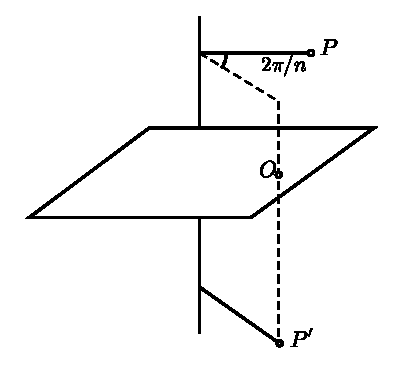
\includegraphics[width=4.2cm]{fig32.pdf}\\[0.3em]{\small 图 32}\end{minipage}\par\nopagebreak
其中 $C_n$ 和 $\sigma_h$ 的操作次序显然对结果无影响.

二阶旋转-反射轴是一个重要的特例.很易看出，转过 $\pi$ 角后再对垂直于转轴的平面反射一次就是一个反演变换，此时物体上的一个 $P$ 点变换到 $PO$ 延线上的 $P'$ 点，并且 $OP$ 等于 $OP'$，$O$ 点为转轴和平面的交点.具有这种变换对称性的物体，称为具有对称中心的物体.我们用记号 $I$ 代表反演操作，故有
\begin{equation}
  I\equiv S_2=C_2\sigma_h.
\end{equation}
显然还有 $I\sigma_h=C_2$，$IC_2=\sigma_h$，换句话说，一个两阶轴、一个垂直于该轴的对称平面以及它们交点处的一个对称中心三者是相互依赖的：只要存在其中的任意两个，第三个也就自动出现.

现在来指出旋转和反射的若干纯几何学性质，这些性质有助于对物体对称性的研究.

转轴交于某点的两个旋转的乘积，等价于绕第三轴的一个旋转，此轴也通过该交点.对两个相交平面的两次反射等价于一个旋转，其转轴显然就是这两个平面的交线，其转角很易用简单的几何作图法求出，它等于两平面夹角的两倍.如果用 $C(\varphi)$ 代表转角为 $\varphi$ 的绕轴旋转，用记号 $\sigma_v$ 和 $\sigma_v'$ 代表\footnote{通常用下标 $v$ 代表对通过某一给定轴的一个平面（“竖直”面）所进行的反射，用下标 $h$ 代表对垂直于该轴的一个平面（“水平”面）所进行的反射.}对通过该轴的两个平面进行的反射，以上的说法即可写成：
\begin{equation}
  \sigma_v\sigma_v'=C(2\varphi),
\end{equation}
式中的 $\varphi$ 是两平面的夹角.必须注意的是，上式中两个反射的乘积次序并不是无所谓的：$\sigma_v\sigma_v'$ 变换给出的旋转方向是从 $\sigma_v'$ 面到 $\sigma_v$ 面，乘积次序对调后给出的旋转具有相反的方向.对 (91.6) 式左乘 $\sigma_v$ 后得
\begin{equation}
  \sigma_v'=\sigma_v C(2\varphi).
\end{equation}
换句话说，旋转操作后再对通过转轴的一个平面反射一次，等价于对另一平面的反射，并且这个反射面和前一平面的夹角等于转角的一半.由此可知，一个两阶对称轴和通过该轴的两个正交对称面是彼此相关的：只要存在其中的两个，第三个也一定存在.

现在来指出，转角为 $\pi$、转轴（图33中的 $Oa$ 和 $Ob$）相交成角 $\varphi$ 的两个旋转，它们的乘积等价于转角为 $2\varphi$、转轴垂直于前两轴（图33中的 $PP'$）的一个旋转.变换的结果仍等于一个旋转是很明显的；经过第一个旋转（绕 $Oa$ 轴）后 $P$ 点变到 $P'$ 点，再经第二个旋转（绕 $Ob$ 轴）后它又回到原位.这就意味着，$PP'$ 直线保持不动，因而是一个转轴.为了求出转角，只要注意到 $Oa$ 轴在第一旋转中保持不动，而经第二旋转后它变到 $Oa'$ 位置，$Oa'$ 和 $Oa$ 的夹角为 $2\varphi$.用同样的方法还可证明，以上两个变换的操作次序对调后所得的旋转具有相反的方向.

\par\nopagebreak\noindent\begin{minipage}{\linewidth}\centering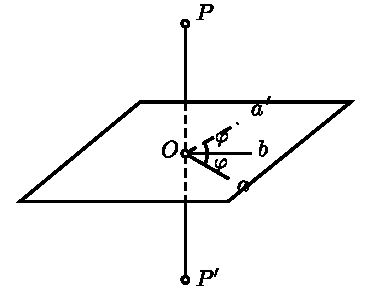
\includegraphics[width=4.2cm]{fig33.pdf}\\[0.3em]{\small 图 33}\end{minipage}\par\nopagebreak

一般讲来两个逐次变换的结果和它们的操作次序有关，但对某些情形也可和操作次序无关：这时我们说两个变换是对易的.以下几种情形就是可对易的变换：

(1) 绕同一轴的两个旋转；

(2) 对正交平面的两个反射（等价于绕其交线旋转 $\pi$ 角）；

(3) 转角为 $\pi$、转轴彼此正交的两个旋转（等价于绕第三个正交轴旋转 $\pi$ 角）；

(4) 一次旋转以及对垂直于转轴的平面所作的一次反射；

(5) 任一旋转（或反射）以及对转轴上（或反射平面上）一个点所作的一次反演.这是根据 (1) 和 (4) 得到的.

\section{变换群}

一个给定物体的所有对称变换的集合，称为该物体的对称变换群（或者简称为对称群）.以上所讲的变换都是指物体的几何变换.但在量子力学的应用中，最好把这些对称变换看作是使该系统的哈密顿量保持不变的各种坐标变换.很明显，如果一个系统经过某一旋转或反射后保持不变，那么它所对应的坐标变换也不会改变该系统的薛定谔方程.因此我们所讲的变换群将是这样的，它使所给的薛定谔方程保持不变\footnote{采用这种观点后不但能包括此处所讲的各种旋转和反射群，而且还能包括保持薛定谔方程不变的其它变换型式.其中包括所考虑系统（分子或原子）中同类粒子间的坐标对换.一个给定系统中同类粒子间所有可能的各种对换的集合，称为该系统的置换群（我们已经在 §63 中碰到过）.以下所讲的群的一般性质对置换群讲来也是适用的，但是我们不准备在这里详述此群.\par 关于本章所用的记号问题，需作下列说明.对称变换实质上都是算符，它和全书所讲的算符是一样的，因此照例要在它的字母上加一个“\textasciicircum{}”号.我们并没有加上这种记号，是由于省略后不会在本章中引起误会，同时和习用的记法相一致.根据同一理由，我们以习用符号 $E$ 代表恒等变换，而不用其它各章中所用的符号 1.最后，反演算符在本章中记作 $I$，而不用 §30 中的 $P$，尽管后者在量子力学新近文献中是常用的.}.

对称群的研究最好是利用群论这一数学工具，它的要点将在下面加以说明.我们先研究含有限多个变换的那种群（称为有限群）.组成该群的每一个变换称为该群的一个群元.

对称群具有以下几点重要性质.所有的群都含有一个恒等变换 $E$（称为该群的单位元）.一个群中的元可以彼此“相乘”，两个（或两个以上）变换的乘积是指这些变换相继施行后所得的最终结果.显然，一个群中任意两元的乘积仍为该群中的一个元.对于群元的乘法，结合律成立：$(AB)C=A(BC)$，其中的 $A,B,C$ 是同一群中的三个元.但是乘法对易律不一定成立：一般讲来，$AB\neq BA$.对群中的每一元 $A$，在同一群中还存在着它的“逆”元 $A^{-1}$（逆变换），满足 $AA^{-1}=E$.在某些情形下，一个元有可能等于它的逆元，特别是 $E^{-1}=E$.互逆元 $A$ 和 $A^{-1}$ 显然是对易的.

两元乘积 $AB$ 的逆元为
\begin{equation*}
  (AB)^{-1}=B^{-1}A^{-1}.
\end{equation*}
更多个元的连乘积也有类似的式子，应用乘法结合律进行相乘后，很易证明这一点.

如果所有的群元全都对易，这样的群称为阿贝尔群.阿贝尔群的一个特例就是循环群.循环群是指这样的群，它的所有元可以表为一个群元的各个逐次乘幂，也就是由下列诸元组成的群：
\begin{equation*}
  A,A^2,A^3,\cdots,A^n=E,
\end{equation*}
$n$ 是某一整数.

设 $\boldsymbol{G}$ 为某一群\footnote{我们用黑斜体拉丁字母代表群.}，如果可以从中取出一组元 $\boldsymbol{H}$，使得 $\boldsymbol{H}$ 本身也构成一个群，那么群 $\boldsymbol{H}$ 就称为群 $\boldsymbol{G}$ 的一个子群.同一个群可以出现在群 $\boldsymbol{G}$ 的不同子群中.

取出群中的任一元 $A$ 进行逐次自乘后，最后可以得到单位元（因为该群的元总数是有限的）.如果 $n$ 是满足 $A^n=E$ 的最小整数，则 $n$ 称为元 $A$ 的阶，同时群元的集合 $A,A^2,\cdots,A^n=E$ 称为 $A$ 的周期.这个周期记作 $\{A\}$，它本身是一个群，也就是原群的一个子群并且是一个循环子群.

要判断所给的一个群元集合是不是一个子群，只要看一下该集合中任意两个元相乘后是不是仍为该集合中的一个元就可以了.事实上，如果该集合是一个子群，集合中每一个元 $A$ 和它的所有自乘幂包括 $A^{n-1}$（$n$ 是这个元的阶）在内都应属于该集合，其中的 $A^{n-1}$ 就是 $A$ 的逆元（因为 $A^{n-1}A=A^n=E$）；单位元显然也在该集合中.

群的元的总数称为该群的阶.很易证明，子群的阶是整群的阶的一个整因子.为此，我们来考虑群 $\boldsymbol{G}$ 的一个子群 $\boldsymbol{H}$，并令 $G_1$ 为群 $\boldsymbol{G}$ 中不属于 $\boldsymbol{H}$ 的某一元.用 $G_1$ 乘（假定为右乘）$\boldsymbol{H}$ 中的所有元，我们得到一组元（称为右陪集）记作 $\boldsymbol{H}G_1$.这个陪集中的所有元显然都属于群 $\boldsymbol{G}$.但是没有一个元属于 $\boldsymbol{H}$，因为如果对 $\boldsymbol{H}$ 中的任意两个元 $H_a$ 和 $H_b$ 有 $H_aG_1=H_b$，就有 $G_1=H_a^{-1}H_b$，这就是说，$G_1$ 也将属于子群 $\boldsymbol{H}$，这是和假设矛盾的.同理可以证明，如果 $G_2$ 是 $\boldsymbol{G}$ 中不属于 $\boldsymbol{H}$ 和 $\boldsymbol{H}G_1$ 的一个元，则陪集 $\boldsymbol{H}G_2$ 中的所有元不能属于 $\boldsymbol{H}$ 和 $\boldsymbol{H}G_1$.继续施行这种手续，最后可把有限群 $\boldsymbol{G}$ 中的所有元全部分尽.所有的元被分成以下诸陪集（$\boldsymbol{G}$ 中 $\boldsymbol{H}$ 的各个陪集）：
\begin{equation*}
  \boldsymbol{H},\boldsymbol{H}G_1,\boldsymbol{H}G_2,\cdots,\boldsymbol{H}G_m,
\end{equation*}
每一个陪集含有 $h$ 个元，$h$ 是子群 $\boldsymbol{H}$ 的阶.由此可见，群 $\boldsymbol{G}$ 的阶 $g$ 为 $g=hm$，定理得证.整数 $m=g/h$ 称为群 $\boldsymbol{G}$ 中子群 $\boldsymbol{H}$ 的指数.

如果群的阶数是一个素数，根据上述定理立刻可知这样的群不存在任何子群（除非是 $E$ 或该群本身）.这个定理的逆命题也是成立的：凡是不存在子群的一个群一定是素数阶并且一定是一个循环群（否则元素的周期将是它的子群）.

现在来引进共轭元这一重要概念.两个元 $A$ 和 $B$ 称为相互共轭的，如果
\begin{equation*}
  A=CBC^{-1},
\end{equation*}
式中的 $C$ 也是该群中的一个元.上式右乘 $C$ 并左乘 $C^{-1}$ 后即得逆式 $B=C^{-1}AC$.共轭元的一个重要特性是，如果 $A$ 共轭于 $B$ 以及 $B$ 共轭于 $C$，就有 $A$ 共轭于 $C$，因从 $B=P^{-1}AP$ 和 $C=Q^{-1}BQ$（$P$ 和 $Q$ 都是该群的元）出发，可得 $C=(PQ)^{-1}A(PQ)$.由于这一点，我们可以讲到由群中的相互共轭元素所组成的一个集合，这样的集合称为该群的一个共轭元类（或简称类）.每一个类完全由该类中的任一个元素 $A$ 所确定：给出 $A$ 后即可作乘积 $GAG^{-1}$，并令 $G$ 依次地等于该群中的各个元，即可得出 $A$ 的整个共轭类（当然，这个办法可能使该类中的每个元得出好几遍）.因此我们可以把整个群分成若干个类，每一个群元显然只能属于其中的一个类.群的单位元本身自成一类，因为对于该群中的所有元，都有 $GEG^{-1}=E$.如果是一个阿贝尔群，每一元都自成一类，因为按定义，所有的群元彼此对易，每一个元只能和自己共轭从而自成一类.要强调的是，群的类（除了 $E$ 这个类）根本不是该群的子群，从它不含单位元这一点就可以看出来.

同一类中的所有元具有相同的阶.实际上，如果 $n$ 是 $A$ 元的阶（因而有 $A^n=E$），那么对它的共轭元 $B=CAC^{-1}$ 就有 $(CAC^{-1})^n=CA^nC^{-1}=E$.

设 $\boldsymbol{H}$ 为群 $\boldsymbol{G}$ 的一个子群，$G_1$ 为 $\boldsymbol{G}$ 中不属于 $\boldsymbol{H}$ 的一个元.很易证明，$G_1\boldsymbol{H}G_1^{-1}$ 这一组元具有群的一切特性，因而也是 $\boldsymbol{G}$ 的一个子群.$\boldsymbol{H}$ 和 $G_1\boldsymbol{H}G_1^{-1}$ 这两个子群称为是共轭的：一个子群中的每个元和另一子群中的一个元相共轭.采取各种不同的 $G_1$，我们得到一系列共轭的子群，其中可能有一部分是彼此重合的.也可能发生这样的情形，凡和 $\boldsymbol{H}$ 共轭的子群都和 $\boldsymbol{H}$ 重合.这种情形下的 $\boldsymbol{H}$ 称为群 $\boldsymbol{G}$ 的一个正规子群或不变子群.例如阿贝尔群的每个子群显然都是它的正规子群.

我们来考虑一个具有 $n$ 个元 $A,A',A'',\cdots$ 的群 $\boldsymbol{A}$，还有一个具有 $m$ 个元 $B,B',B'',\cdots$ 的群 $\boldsymbol{B}$，并且假定 $\boldsymbol{A}$ 的所有元（除了单位元 $E$ 外）都不同于 $\boldsymbol{B}$ 的元但和 $\boldsymbol{B}$ 的元相对易.如果把群 $\boldsymbol{A}$ 的每个元和群 $\boldsymbol{B}$ 的每个元相乘起来，可以得到 $nm$ 个元，它们也组成一个群.实际上，其中的任意两个元相乘后 $AB\cdot A'B'=AA'\cdot BB'=A''B''$ 仍为其中的一个元.所得的 $nm$ 阶群记作 $\boldsymbol{A}\otimes\boldsymbol{B}$，并称为群 $\boldsymbol{A}$ 和 $\boldsymbol{B}$ 的直积.

最后来介绍群的同构概念.两个同阶的群 $\boldsymbol{A}$ 和 $\boldsymbol{B}$，如果在双方的元间可以建立起某种一一对应关系，使得元 $A$ 对应于元 $B$ 以及元 $A'$ 对应于元 $B'$ 时，就有元 $A''=AA'$ 对应于元 $B''=BB'$，则这两个群就称为同构的.这样的两个群从抽象观点看来显然具有相同的性质，尽管它们的元具有不同的实际含义.

\section{点群}

有限大物体（例如一个分子）的对称群必须是这样的，该物体上至少要有一个点对群中的任一变换都保持不变.换句话说，一个分子的所有对称轴和所有对称平面至少要有一个公共交点.实际上，绕两个不相交轴的逐次旋转或者对两个不相交平面的逐次反射都能使物体发生位移，从而不能使该物体与原先重合.具有以上性质的对称群就称为点群.

在构造点群的各种可能类型之前，我们先介绍一个简单的几何手续，以便对一个群的诸元进行分类.设 $Oa$ 为某一轴线，$A$ 为绕该轴旋转某个定角的一个群元.并设 $G$ 为同一群中的一个变换（旋转或反射），它把 $Oa$ 轴变到 $Ob$ 位置.现在来证明 $B=GAG^{-1}$ 元相当于绕 $Ob$ 轴的一个旋转，它的转角等于 $A$ 元绕 $Oa$ 轴的转角.为此，可以考虑 $GAG^{-1}$ 变换作用于 $Ob$ 轴本身的结果.$G$ 的逆变换 $G^{-1}$ 先把 $Ob$ 轴变到 $Oa$ 位置，下一步的 $A$ 变换使该轴保持不动，最后的 $G$ 变换又使该轴回到原来位置.最后结果是 $Ob$ 轴保持不变，因而 $B$ 变换就是绕该轴的一个旋转.由于 $A$ 和 $B$ 属于同一共轭类，具有相同的阶，这就意味着它们的转角相同.

由此得出结论，转角相同的两个旋转是属于同一类的，如果该群中存在一个元能把一个转轴变到另一个转轴的话.用同样方法还可以证明，如果该群中存在一个变换能把一个平面变到另一个平面的话，那么对不同平面的两个反射是属于同一类的.至于那些可以相互变换的对称轴或对称平面，则称为等价的.

以上所讲的两个旋转如果是绕同一轴的，还需作某些补充说明.设 $C_n^k\ (k=1,2,\cdots,n-1)$ 是绕某一 $n$ 阶对称轴的各个旋转元，$C_n^k$ 的逆元 $C_n^{-k}=C_n^{n-k}$ 等于绕同一方向转过 $(n-k)(2\pi/n)$ 角，也等于逆向转过 $2k\pi/n$ 角.如果该群中存在一个绕其垂直轴旋转 $\pi$ 角的变换（这个变换能使 $n$ 阶轴反向），那么根据上段所讲的一般规则，$C_n^k$ 和 $C_n^{-k}$ 将属于同类.对垂直于该轴的平面所作的一次反射 $\sigma_h$ 也能使该轴（$n$ 阶轴）反向，但是必须注意，这样的反射还能改变旋转的方向.因此 $\sigma_h$ 的存在并不能使 $C_n^k$ 和 $C_n^{-k}$ 共轭.另一方面，对通过该轴的平面所作的一次反射 $\sigma_v$ 并不能改变该轴的方向但能改变旋转的方向，因此有 $C_n^{-k}=\sigma_vC_n^k\sigma_v$.如果有这样的对称面存在，$C_n^k$ 和 $C_n^{-k}$ 就属于同类.如果转轴和转角相同但旋转方向不同的两个元是共轭的，该转轴就称为双向轴.

点群的分类还常用到下列规则.设 $\boldsymbol{G}$ 是不含反演 $I$ 的群，$\boldsymbol{C}_i$ 是由 $I$ 和 $E$ 两个元组成的群.则直积 $\boldsymbol{G}\otimes\boldsymbol{C}_i$ 是一个群，它含有两倍于 $\boldsymbol{G}$ 的元，其中的一半元等于 $\boldsymbol{G}$ 群的元，另一半元是由后者乘以 $I$ 后得到的.由于 $I$ 和点群的任意其它变换都对易，显然群 $\boldsymbol{G}\otimes\boldsymbol{C}_i$ 具有两倍于 $\boldsymbol{G}$ 的类：$\boldsymbol{G}$ 群中的每一个类 $A$ 对应于群 $\boldsymbol{G}\otimes\boldsymbol{C}_i$ 中 $A$ 和 $AI$ 两个类.特别是，反演 $I$ 总是自成一类.

现在可以历数所有可能的各种点群.我们来构造这些点群，先从最简单的开始然后逐步加入新的对称元.我们用黑斜体的拉丁字母附上适当的下标代表这些点群.

\subsection*{I.\ 群 $\boldsymbol{C}_n$}

这是最简单的对称型式，它只有一个 $n$ 阶对称轴.$\boldsymbol{C}_n$ 群就是绕 $n$ 阶轴旋转的群.这个群显然是一个循环群.它的 $n$ 个元各自形成一类.$\boldsymbol{C}_1$ 群只含恒等变换 $E$，相当于不存在任何对称性的情形.

\subsection*{II.\ 群 $\boldsymbol{S}_{2n}$}

$\boldsymbol{S}_{2n}$ 群是绕一个 $2n$（偶数）阶旋转-反射轴的旋转反射群.它含有 $2n$ 个元并且显然是一个循环群.特别是 $\boldsymbol{S}_2$ 群，它只含 $E$ 和 $I$ 两个元素，这个群又记作 $\boldsymbol{C}_i$.要指出的是，如果群的阶数取 $2n=4p+2$ 的形式，元中就含有反演，因为 $(S_{4p+2})^{2p+1}=C_2\sigma_h=I$.这样的群可以写成直积形式：$\boldsymbol{S}_{4p+2}=\boldsymbol{C}_{2p+1}\otimes\boldsymbol{C}_i$，也记作 $\boldsymbol{C}_{2p+1,i}$.

\subsection*{III.\ 群 $\boldsymbol{C}_{nh}$}

这种群是由一个 $n$ 阶对称轴加进一个垂直于它的对称平面后得到的.$\boldsymbol{C}_{nh}$ 群含有 $2n$ 个元：其中有 $\boldsymbol{C}_n$ 群的 $n$ 个旋转以及 $n$ 个旋转-反射变换 $C_n^k\sigma_h,\ k=1,2,\cdots,n$（其中包括反射 $C_n^n\sigma_h=\sigma_h$）.这个群的所有元是对易的，即它是一个阿贝尔群，它的类数等于元数.如果 $n$ 为偶数 $(n=2p)$，这个群含有一个对称中心（因为 $C_{2p}^p\sigma_h=C_2\sigma_h=I$）.最简单的群 $\boldsymbol{C}_{1h}$ 只含 $E$ 和 $\sigma_h$ 两个元素，它又记作 $\boldsymbol{C}_s$.

\subsection*{IV.\ 群 $\boldsymbol{C}_{nv}$}

如果一个 $n$ 阶对称轴再加进一个通过该轴的对称平面，就会自动地得出另外 $n-1$ 个通过该轴的夹角为 $\pi/n$ 的对称平面［根据 §91 中所讲的几何定理 (91.7)\footnote{很易证明，有限群中两个对称平面的夹角不可能不等于 $2\pi$ 的一个有理分式.否则的话，这种对称面进行无限反复的相互反射后，就会得到无限多个相交于同一轴线的对称平面.换句话说，只要存在两个这样的平面，就会导致整个的轴对称.}］.由此而得的群 $\boldsymbol{C}_{nv}$ 含有 $2n$ 个元：绕 $n$ 阶轴的 $n$ 个旋转以及对竖直面的 $n$ 个反射 $\sigma_v$.图 34 中画出了 $\boldsymbol{C}_{3v}$ 群和 $\boldsymbol{C}_{4v}$ 群的对称平面和对称轴线.

\par\nopagebreak\noindent\begin{minipage}{\linewidth}\centering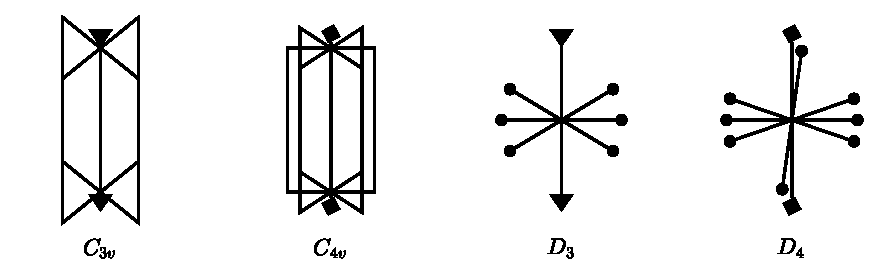
\includegraphics[width=9.5cm]{fig34.pdf}\\[0.3em]{\small 图 34}\end{minipage}\par\nopagebreak

确定其类时，我们注意到，由于存在着通过轴线的对称平面，这个轴是双向的.群元在各类中的具体分布取决于 $n$ 是偶数还是奇数.

如果 $n$ 是奇数 $(n=2p+1)$，每一个平面经过逐次的旋转 $C_{2p+1}$ 后可以依次地变到其它的 $2p$ 个平面，因此所有的对称平面都是等价的，对它们的反射属于同一类.绕轴的旋转中除了恒等变换外共有 $2p$ 个操作并且成对地共轭.所以它们组成 $p$ 个类，每类有两个元（$C_{2p+1}^k$ 和 $C_{2p+1}^{-k},\ k=1,2,\cdots,p$）.此外 $E$ 自成一类.因此总共有 $p+2$ 类.

如果 $n$ 是偶数 $(n=2p)$，逐次旋转 $C_{2p}$ 只能使相间平面相互变换，两个相邻平面无法相互变换.因而存在两组等价面，每组有 $p$ 个，相应地就有两个类，每个类有 $p$ 个元（反射元）.在绕轴的旋转中，$C_{2p}^{2p}=E$ 和 $C_{2p}^p=C_2$ 各自组成一类，其余的 $2p-2$ 个旋转成对地共轭并给出 $p-1$ 个类，每类有两个元.因此群 $\boldsymbol{C}_{2p,v}$ 共有 $p+3$ 个类.

\subsection*{V.\ 群 $\boldsymbol{D}_n$}

一个 $n$ 阶对称轴如果再加进一个垂直于它的二阶对称轴，就会自动地产生 $n-1$ 个另外的二阶对称轴，因此共有 $n$ 个夹角为 $\pi/n$ 的二阶水平轴.结果所得的群 $\boldsymbol{D}_n$ 含有 $2n$ 个元：绕 $n$ 阶轴的 $n$ 个旋转以及绕水平轴转 $\pi$ 角的 $n$ 个旋转（我们用 $U_2$ 代表这种旋转，保留 $C_2$ 代表绕竖直轴转 $\pi$ 角的旋转）.作为例子，图 34 画出了群 $\boldsymbol{D}_3$ 和 $\boldsymbol{D}_4$ 的对称轴系.

和情形 IV 一样，我们可以证明 $n$ 阶轴是一个双向轴.当 $n$ 是奇数时，所有的二阶水平轴都是等价的；当 $n$ 是偶数时，它们组成两个不等价的集合.因此群 $\boldsymbol{D}_{2p}$ 共有 $p+3$ 个类：$E$，两个 $U_2$ 类每类含有 $p$ 个旋转 $U_2$，旋转 $C_2$，还有 $p-1$ 类每类含有两个绕竖直轴的旋转.另一方面，群 $\boldsymbol{D}_{2p+1}$ 却有 $p+2$ 类：$E$，$2p+1$ 个旋转 $U_2$，还有 $p$ 类每类含有绕竖直轴的两个旋转.

群 $\boldsymbol{D}_2$ 是一个重要的特例.它的对称轴系是由三个相互正交的二阶轴组成的.这个群也记作 $\boldsymbol{V}$.

\subsection*{VI.\ 群 $\boldsymbol{D}_{nh}$}

如果在群 $\boldsymbol{D}_n$ 的轴系中再加进一个水平对称面通过 $n$ 个二阶轴，就会自动地出现 $n$ 个竖直平面，每个平面通过竖直轴和一个水平轴.由此而得的 $\boldsymbol{D}_{nh}$ 群含有 $4n$ 个元素：除了 $\boldsymbol{D}_n$ 群的 $2n$ 个元素外还有 $n$ 个反射 $\sigma_v$ 和 $n$ 个旋转-反射变换 $C_n^k\sigma_h$.图 35 中画出了 $\boldsymbol{D}_{3h}$ 群的对称轴和对称面.

\par\nopagebreak\noindent\begin{minipage}{\linewidth}\centering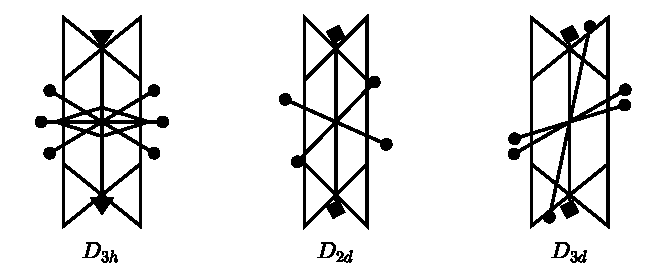
\includegraphics[width=9.5cm]{fig35.pdf}\\[0.3em]{\small 图 35}\end{minipage}\par\nopagebreak

反射 $\sigma_h$ 和此群的所有其它元都对易，因此可把 $\boldsymbol{D}_{nh}$ 写作直积 $\boldsymbol{D}_{nh}=\boldsymbol{D}_n\otimes\boldsymbol{C}_s$，其中的 $\boldsymbol{C}_s$ 是由 $E$ 和 $\sigma_h$ 两个元组成的群.当 $n$ 为偶数时，群元中含有反演操作，因此还可写成 $\boldsymbol{D}_{2p,h}=\boldsymbol{D}_{2p}\otimes\boldsymbol{C}_i$.

由此可知，$\boldsymbol{D}_{nh}$ 群的类数两倍于 $\boldsymbol{D}_n$ 群的类数.其中的一半和 $\boldsymbol{D}_n$ 群的类相同（绕轴旋转），其余的一半是由前者乘以 $\sigma_h$ 后得到的.对竖直面的反射 $\sigma_v$ 都属于一类（如果 $n$ 是奇数）或者组成两类（如果 $n$ 是偶数），旋转-反射变换 $\sigma_hC_n^k$ 和 $\sigma_hC_n^{-k}$ 成对共轭.

\subsection*{VII.\ 群 $\boldsymbol{D}_{nd}$}

还可以用另一种方式在 $\boldsymbol{D}_n$ 群的轴系中加进对称平面.所加进的竖直面通过 $n$ 阶轴并且平分两个相邻二阶水平轴的夹角.加进这样的一个平面后又会自动产生其它 $n-1$ 个竖直平面.由此而得的对称平面系和对称轴系确定了群 $\boldsymbol{D}_{nd}$（图 35 中画出了群 $\boldsymbol{D}_{2d}$ 和群 $\boldsymbol{D}_{3d}$ 的平面系和轴系）.

群 $\boldsymbol{D}_{nd}$ 含有 $4n$ 个元.除了群 $\boldsymbol{D}_n$ 的 $2n$ 个元外，要加上对竖直面的 $n$ 个反射（记作 $\sigma_d$，$d$ 表示“对角”平面）以及具有形式为 $G=U_2\sigma_d$ 的 $n$ 个变换.为了弄清变换 $G$ 的性质，我们注意到，根据 (91.6) 式旋转 $U_2$ 可以表成 $U_2=\sigma_h\sigma_v$ 的形式，式中的 $\sigma_v$ 是对通过二阶轴的竖直面的反射.因此 $G=\sigma_h\sigma_v\sigma_d$（$\sigma_v$ 和 $\sigma_h$ 变换本身当然不是该群的元）.由于 $\sigma_v$ 和 $\sigma_d$ 的反射面相交于 $n$ 阶轴，夹角为 $(2k+1)\pi/2n,\ k=1,\cdots,(n-1)$（由于相邻面的夹角为 $\pi/2n$），根据 (91.6) 式就有 $\sigma_v\sigma_d=C_{2n}^{2k+1}$.因此得 $G=\sigma_hC_{2n}^{2k+1}=S_{2n}^{2k+1}$，因此这些元就是绕竖直轴的旋转-反射变换.由此可见，这个竖直轴不是一个简单的 $n$ 阶对称轴，而是一个 $2n$ 阶旋转-反射轴.

对角平面使两个相邻的二阶水平轴相互反射，故在该群中相邻的二阶轴是等价的（$n$ 是奇数或偶数时都成立）.同理，所有的对角平面也是等价的.旋转-反射变换 $S_{2n}^{2k+1}$ 和 $S_{2n}^{-2k-1}$ 成对地共轭\footnote{因为
\begin{equation*}
  \sigma_d S_{2n}^{2k+1}\sigma_d=\sigma_d\sigma_h C_{2n}^{2k+1}\sigma_d=\sigma_h\sigma_d C_{2n}^{2k+1}\sigma_d=\sigma_h C_{2n}^{-2k-1}=S_{2n}^{-2k-1}.
\end{equation*}}.

把以上的考虑应用到群 $\boldsymbol{D}_{2p,d}$，我们发现它共有以下的 $2p+3$ 类：$E$，绕 $n$ 阶轴的旋转 $C_2$，绕 $n$ 阶轴的其余旋转组成的 $p-1$ 类每类含有两个共轭的旋转，$2p$ 个旋转 $U_2$ 组成的一个类，$2p$ 个反射 $\sigma_d$ 组成的一个类，还有 $p$ 类每类含有两个旋转-反射变换.

当 $n$ 为奇数时 $(n=2p+1)$，群元中含有反演（因为此时有一个水平轴和一个垂直面正交）.因而可以写成 $\boldsymbol{D}_{2p+1,d}=\boldsymbol{D}_{2p+1}\otimes\boldsymbol{C}_i$，可见 $\boldsymbol{D}_{2p+1,d}$ 群共有 $2p+4$ 个类，这些类可以由 $\boldsymbol{D}_{2p+1}$ 群的 $p+2$ 个类直接求出.

\subsection*{VIII.\ 群 $\boldsymbol{T}$（四面体群）}

这个群的轴系等于一个正四面体的对称轴系.它可以由群 $\boldsymbol{V}$ 的轴系中加进四条三阶斜轴得到，绕三阶斜轴旋转时可使三条二阶轴相互变换.这套轴系也可利用正立方体表出，三条二阶轴为正立方体三对平行面的面心联线，三阶轴为该立方体的斜对角线.图 36 中画出了这些轴线在正立方体以及在正四面体中的位置（每种轴线只画出一条）.

三条二阶轴是彼此等价的.四条三阶轴也是等价的，因为它们可以通过 $C_2$ 旋转而相互易位，但它们不是双向轴.由此可知，$\boldsymbol{T}$ 群共有 12 个元分成四类：$E$，三个 $C_2$ 旋转，四个 $C_3$ 旋转和四个 $C_3^2$ 旋转.

\par\nopagebreak\noindent\begin{minipage}{\linewidth}\centering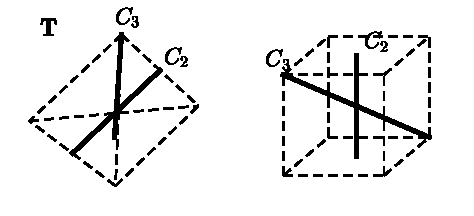
\includegraphics[width=7cm]{fig36.pdf}\\[0.3em]{\small 图 36}\end{minipage}\par\nopagebreak

\subsection*{IX.\ 群 $\boldsymbol{T}_d$}

这个群包括了正四面体的所有对称变换，它的轴系可以从群 $\boldsymbol{T}$ 轴系中加进对称平面而得到，每一个对称平面通过一条二阶轴和两条三阶轴.从而使二阶轴变为四阶旋转-反射轴（和 $\boldsymbol{D}_{2d}$ 中的情形相似）.这套对称系统可简便地用下面的方式表达：三条旋转-反射轴各通过正立方体 3 对平行面的面心，四条三阶轴是该立方体的斜对角线，六个对称平面各通过该立方体的六对平行边（图 37 中画出了每种轴线中的一条和一个平面）.

\par\nopagebreak\noindent\begin{minipage}{\linewidth}\centering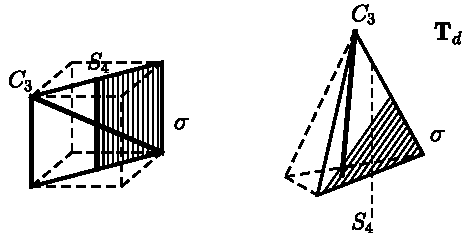
\includegraphics[width=7cm]{fig37.pdf}\\[0.3em]{\small 图 37}\end{minipage}\par\nopagebreak

由于对称面通过三阶轴，这些轴都是双向轴.同种的所有轴线和同种的所有平面都是等价的.因而这个群的 24 个元分成以下五类：$E$；8 个 $C_3$ 和 $C_3^2$ 旋转；6 个对称平面的反射；6 个 $S_4$ 和 $S_4^3$ 旋转-反射变换以及 3 个 $C_2=S_4^2$ 旋转.

\subsection*{X.\ 群 $\boldsymbol{T}_h$}

这个群是由群 $\boldsymbol{T}$ 加进一个对称中心后得到的，即 $\boldsymbol{T}_h=\boldsymbol{T}\otimes\boldsymbol{C}_i$.结果出现三个相互正交的对称平面，每个平面通过一对二阶轴，并使三阶轴变成六阶旋转-反射轴（图 38 中画出了每种轴线中的一条和一个平面）.

这个群含有 24 个元并分为 8 类，它们可以从群 $\boldsymbol{T}$ 的类直接求得.

\par\nopagebreak\noindent\begin{minipage}{\linewidth}\centering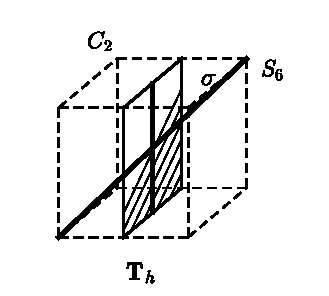
\includegraphics[width=5.5cm]{fig38.pdf}\\[0.3em]{\small 图 38}\end{minipage}\par\nopagebreak

\subsection*{XI.\ 群 $\boldsymbol{O}$（八面体群）}

这个群的轴系是一个正立方体的对称轴系.计有 3 条四阶轴通过对面的面心，4 条三阶轴通过对顶角，6 条二阶轴通过相对的棱的中点（图 39）.

很易看出，所有的同阶轴是等价的，而且每个轴都是双向轴.因此 24 个元分成以下五类：$E$；8 个 $C_3$ 和 $C_3^2$ 旋转；6 个 $C_4$ 和 $C_4^3$ 旋转；3 个 $C_4^2$ 旋转以及 6 个 $C_2$ 旋转.


\subsection*{XII.\ 群 $\boldsymbol{O}_h$}

这是正立方体所有对称变换所组成的群\footnote{群 $\boldsymbol{T}$，$\boldsymbol{T}_d$，$\boldsymbol{T}_h$，$\boldsymbol{O}$，$\boldsymbol{O}_h$ 常称为立方体群}.可从群 $\boldsymbol{O}$ 加进一个对称中心得到：$\boldsymbol{O}_h=\boldsymbol{O}\otimes\boldsymbol{C}_i$.群 $\boldsymbol{O}$ 的三阶轴因此变成了六阶旋转-反射轴（正立方体的空间对角线），此外还出现 6 个对称面，通过每一对平行边，还有三个平行于立方体各面的平面（图 40）.这个群共有 48 个元分成 10 类，它们可以从群 $\boldsymbol{O}$ 的类直接求得.5 个类和群 $\boldsymbol{O}$ 的相同，其余的 5 类是：$I$；8 个 $S_6$ 和 $S_6^5$ 旋转-反射变换；6 个绕四阶轴的旋转-反射变换 $C_4\sigma_h$ 和 $C_4^3\sigma_h$；3 个对四阶水平面的反射 $\sigma_h$ 以及 6 个对四阶轴垂直面的反射 $\sigma_v$.

\par\nopagebreak\noindent\begin{minipage}{\linewidth}\centering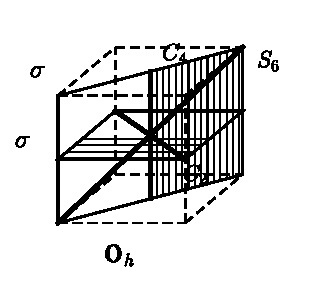
\includegraphics[width=5.5cm]{fig40.pdf}\\[0.3em]{\small 图 40}\end{minipage}\par\nopagebreak

\subsection*{XIII, XIV.\ 群 $\boldsymbol{Y}$, $\boldsymbol{Y}_h$（二十面体群）}

这两个群物理上并不重要，因为自然界并不存在这样的分子对称群.我们就简单地提一下，群 $\boldsymbol{Y}$ 是绕正二十面体（表面为二十个正三角形的凸体）或正十二面体（表面为十二个正五边形的凸体）对称轴系的 60 个旋转所组成的群，计有 6 个五阶轴 10 个三阶轴和 15 个两阶轴.$\boldsymbol{Y}_h$ 群是加入对称中心后得到的，$\boldsymbol{Y}_h=\boldsymbol{Y}\otimes\boldsymbol{C}_i$，它是以上正多面体的所有对称变换组成的群.

以上列举了元数为有限的所有类型的点群.此外尚需考虑元数为无限的连续点群.它将在 §98 中讨论.

\section{群的表示}

我们来考虑任一对称群，设 $\psi_1$ 为所考虑物理系统位形空间中的某个坐标单值函数.在对应于群元 $G$ 的坐标变换下，这个函数变成另一个函数.考虑到该群中的 $g$ 个变换（$g$ 是该群的阶），一般讲来可从 $\psi_1$ 出发得到 $g$ 个不同的函数.对于某种 $\psi_1$ 讲来，其中的某些函数可能是线性相关的.结果可以得到 $f$ 个 $(f\leqslant g)$ 线性独立的函数 $\psi_1,\psi_2,\cdots,\psi_f$，它们在该群所属的各种变换下变为它们之间的线性组合.换句话说，$G$ 变换的结果使每个 $\psi_i$ 函数 $(i=1,2,\cdots,f)$ 变成下列线性组合：
\begin{equation*}
  \sum_{k=1}^{f}G_{ki}\psi_k,
\end{equation*}
式中的 $G_{ki}$ 是一些依赖于变换 $G$ 的常数.这些常数的集合组成变换矩阵\footnote{由于 $\psi_i$ 函数都是单值的，该群中的每个元和一个特定的变换矩阵相对应.}.

根据上述关系，我们最好把群元 $G$ 看成是作用在函数 $\psi_i$ 上的算符，从而可写作：
\begin{equation}
  \hat{G}\psi_i=\sum_k G_{ki}\psi_k.
\end{equation}

\par\nopagebreak\noindent\begin{minipage}{\linewidth}\centering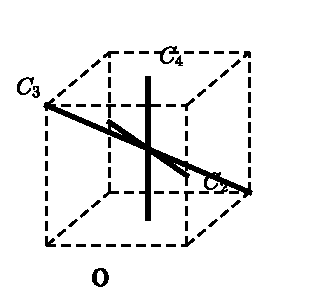
\includegraphics[width=5.5cm]{fig39.pdf}\\[0.3em]{\small 图 39}\end{minipage}\par\nopagebreak
函数组 $\psi_i$ 总可以选成是正交归一化的函数组.此时变换矩阵的概念就和 §11 中所定义的算符矩阵概念相一致，它的矩阵元为：
\begin{equation}
  G_{ik}=\int\psi_i^{*}\hat{G}\psi_k\,\mathrm{d}q.
\end{equation}
两个群元 $G$ 和 $H$ 的乘积，对应于矩阵 $G$ 和矩阵 $H$ 用通常的矩阵乘法法则 (11.12) 相乘后所得的矩阵：
\begin{equation}
  (GH)_{ik}=\sum_l G_{il}H_{lk}.
\end{equation}
与所有的群元分别对应的各矩阵的集合，称为该群的一个表示.定义这些矩阵时所用的函数 $\psi_1,\cdots,\psi_f$ 称为这个表示的基函数.这些函数的总数 $f$ 称为该表示的维数.

我们来考虑积分 $\int\psi_i^{*}\psi_k\,\mathrm{d}q$.由于积分延及整个空间，积分值对坐标系的任意旋转或反射显然保持不变，这就是说，对称变换不会破坏基函数的正交归一化性质，从而 $\hat{G}$ 都是么正算符\footnote{这个论断中重要的是，积分值或者为零（$i\neq k$ 时）或者肯定不为零（$i=k$ 时），因为被积函数 $|\psi_i|^2$ 是正的.}（见 §12），因此，在以正交归一化函数组为基的一个表示中，代表群元的矩阵也都是幺正矩阵.

假定对函数组 $\psi_1,\cdots,\psi_f$ 施行下列线性幺正变换：
\begin{equation}
  \psi_i'=\hat{S}\psi_i,
\end{equation}
所得的新函数组 $\psi_1',\cdots,\psi_f'$ 仍然是正交归一化的（参考 §12）\footnote{按（12.12）式，变换的么正性使得基函数组的模量平方之和在变换中保持不变.}.如果现在取函数组 $\psi_i'$ 为表示的基函数组，我们得到一个维数相同的新表示.这种通过基函数组的相互线性变换而得到的表示，称为等价表示.这些相互等价的表示显然没有本质的区别.

等价表示的矩阵可以简单地相互表达.根据 (12.7) 式，算符 $\hat{G}$ 在新表示中的矩阵，等于下列算符在旧表示中的矩阵：
\begin{equation}
  \hat{G}'=\hat{S}^{-1}\hat{G}\hat{S}.
\end{equation}
代表群元 $G$ 的矩阵中，对角元之和（即阵迹）称为群元的特征标，我们把它记作 $\chi(G)$.一个极为重要的结论是，等价表示的矩阵具有相同的特征标（见 (12.11) 式）.这就显示了利用特征标描述群表示的特殊重要性：它可以立即区别等价的表示和根本不同的表示.以后我们只把不等价的表示称为不同的表示.

如果我们把 (94.5) 中的 $S$ 看作一个群元，它联系着共轭元 $G$ 和 $G'$，即可得出这样的结论，在群的任一给定表示中，属于同一类的群元具有相同的特征标.

恒等变换对应于群的单位元 $E$.单位元的矩阵在所有的表示中都是对角的，且对角元都等于 1.因此特征标 $\chi(E)$ 正好等于该表示的维数：
\begin{equation}
  \chi(E)=f.
\end{equation}
我们来考虑某一 $f$ 维的表示.有可能发生这样的情形，经过 (94.4) 式的适当线性组合以后，它的基函数可以分成若干组，每组分别具有 $f_1,f_2,\cdots$ 个函数（$f_1+f_2+\cdots=f$），当群中的任一元作用在这些函数上时，各组的函数只能变成本组的各函数的线性组合而不能变成其它组的函数.在这样的情形下，所考虑的表示称为可约表示.

另一方面，如果一组基函数不管进行怎样的线性组合，在群元的作用下它的总数不能分解或减少，由这组函数所给出的表示就称为不可约表示.任一可约表示都能分解成为若干个不可约表示.这就是说，经过适当的线性组合以后，它的基函数可以分解成为若干个组，每一组函数在群元的作用下按某一不可约表示变换.其中若干个不同的组也有可能按同一不可约表示变换.在这种情况下，我们就说可约表示中含有这种不可约表示若干次.

不可约表示是群的重要特征，它在群论的所有量子力学应用中都占有主要地位.下面给出不可约表示的若干基本性质\footnote{这些性质的证明可以在任何一本群论教科书中找到.}.

可以证明，一个群的不等价不可约表示的数目等于该群的类数 $r$.我们用不同的号码来区别各种不可约表示的特征标.群元素 $G$ 在这些表示中的特征标分别记作 $\chi^{(1)}(G),\chi^{(2)}(G),\cdots,\chi^{(r)}(G)$.

不可约表示的矩阵元满足一系列正交关系.首先，对于两个不等价的不可约表示，下列关系式成立：
\begin{equation}
  \sum_G G_{ik}^{(\alpha)}G_{lm}^{(\beta)}{}^{*}=0,
\end{equation}
式中的 $\alpha\neq\beta$ 区别两个不可约表示，$\sum_G$ 代表对该群的所有元求和.对于同一个不可约表示，下式成立：
\begin{equation}
  \sum_G G_{ik}^{(\alpha)}G_{lm}^{(\alpha)}{}^{*}
  =\frac{g}{f_\alpha}\delta_{il}\delta_{km},
\end{equation}
也就是说，只有矩阵元的模量平方和才不等于零：
\begin{equation*}
  \sum_G\bigl|G_{ik}^{(\alpha)}\bigr|^2=\frac{g}{f_\alpha}.
\end{equation*}
(94.7) 和 (94.8) 式可以合并写成下列形式：
\begin{equation}
  \sum_G G_{ik}^{(\alpha)}G_{lm}^{(\beta)}{}^{*}
  =\frac{g}{f_\alpha}\delta_{\alpha\beta}\delta_{il}\delta_{km}.
\end{equation}
特别是，从上式出发可求出不可约表示特征标的一个重要的正交关系.(94.9) 式两边对 $i=k,l=m$ 的各个值求和后可得
\begin{equation}
  \sum_G\chi^{(\alpha)}(G)\chi^{(\beta)}(G)^{*}=g\delta_{\alpha\beta},
\end{equation}
$\alpha=\beta$ 时有
\begin{equation*}
  \sum_G\bigl|\chi^{(\alpha)}(G)\bigr|^2=g.
\end{equation*}
这就是说，一个不可约表示的特征标的模量平方和等于该群的阶数.要注意的是，上式可以作为一个判据，用来判断一个表示是不是不可约表示.对于一个可约表示，上式右边的和总是大于 $g$（例如等于 $ng$，$n$ 是该可约表示中所含的不可约表示数）.

由 (94.10) 式还可得出，两个不可约表示具有相同的特征标不但是这两个表示为等价的必要条件而且也是充分条件.

由于同类元的特征标相同，(94.10) 的求和中实际上只有 $r$ 个独立项，该式可写成下列形式
\begin{equation}
  \sum_C g_C\chi^{(\alpha)}(C)\chi^{(\beta)}(C)^{*}=g\delta_{\alpha\beta},
\end{equation}
式中是对该群的 $r$ 个类（用巡标 $C$ 表示）求和，$g_C$ 是 $C$ 类中元的个数.

因不可约表示的个数等于类数，$r^2$ 个量 $f_{\alpha C}=\sqrt{g_C/g}\,\chi^{(\alpha)}(C)$ 可以组成一个方矩阵.

根据对第一个下标的正交式
\begin{equation*}
  \sum_C f_{\alpha C}f_{\beta C}^{*}=\delta_{\alpha\beta},
\end{equation*}
可以自动得出对第二个下标的正交式
\begin{equation*}
  \sum_\alpha f_{\alpha C}f_{\alpha C'}^{*}=\delta_{CC'}.
\end{equation*}
因此除了 (94.11) 式以外，还有
\begin{equation}
  \sum_\alpha\chi^{(\alpha)}(C)\chi^{(\alpha)}(C')^{*}
  =\frac{g}{g_C}\delta_{CC'}.
\end{equation}
任一个群的各种不可约表示中，总是存在一个平凡的不可约表示，它只有一个基函数，这个函数在群的所有变换下保持不变.这个一维表示称为单位表示，该表示中的所有特征标都等于 1.如果正交关系 (94.10) 或 (94.11) 中有一个是单位表示，则对另一个表示有
\begin{equation}
  \sum_G\chi^{(\alpha)}(G)=\sum_C g_C\chi^{(\alpha)}(C)=0.
\end{equation}
这就是说，对于每一个不可约表示，所有群元的特征标之和等于零.

根据 (94.10) 式，我们很容易把任一可约表示分解成不可约表示，只要这些表示的特征标是已知的.设 $\chi(G)$ 为某个 $f$ 维可约表示的特征标，并令整数 $a^{(1)},a^{(2)},\cdots,a^{(r)}$ 分别代表该表示中所含的各个不可约表示的次数，因而有
\begin{equation}
  \sum_{\beta=1}^{r}a^{(\beta)}f_\beta=f,
\end{equation}
式中 $f_\beta$ 是不可约表示的维数.特征标 $\chi(G)$ 则可写成
\begin{equation}
  \chi(G)=\sum_{\beta=1}^{r}a^{(\beta)}\chi^{(\beta)}(G).
\end{equation}
上式乘以 $\chi^{(\alpha)}{}^{*}(G)$ 并对所有的 $G$ 求和，根据 (94.10) 式得
\begin{equation}
  a^{(\alpha)}=\frac{1}{g}\sum_G\chi(G)\chi^{(\alpha)}(G)^{*}.
\end{equation}
我们来考虑一个 $f=g$ 维的表示，它由 $g$ 个函数 $\hat{G}\psi$ 给出，$\psi$ 是坐标的一般函数（因而由 $\psi$ 所得的 $g$ 个函数 $\hat{G}\psi$ 彼此线性独立），这样的表示称为正规表示.很明显在这个表示中，除了单位元所对应的矩阵外没有一个矩阵含有不等于零的对角矩阵元.因而有 $G\neq E$ 时 $\chi(G)=0$ 以及 $\chi(E)=g$.把这个表示分解成为不可约表示，根据 (94.16) 式，整数 $a^{(\alpha)}$ 的数值为 $a^{(\alpha)}=(1/g)gf^{(\alpha)}=f^{(\alpha)}$.也就是说，每个不可约表示在正规表示中所含的次数等于它的维数.把 $a^{(\alpha)}=f^{(\alpha)}$ 代入 (94.14) 式即得下列关系式：
\begin{equation}
  f_1^2+f_2^2+\cdots+f_r^2=g,
\end{equation}
即一个群的所有不可约表示的维数平方之和等于该群的阶数\footnote{可以提及的是，对点群讲来，当 $r$ 和 $g$ 给定后，实际上只能有一组整数值 $f_1,\cdots,f_r$ 可以满足（94.17）式.}.由此可见，对于一个阿贝尔群（此时 $r=g$），所有的不可约表示都是一维的（$f_1=f_2=\cdots=f_r=1$）.

我们还可以不加证明地指出，不可约表示的维数可以除尽该群的阶数 $g$.

实际上，我们可以通过下式把一个正规表示分解成不可约部分：
\begin{equation}
  \psi_i^{(\alpha)}=\frac{f_\alpha}{g}\sum_G G_{ik}^{(\alpha)}{}^{*}\hat{G}\psi.
\end{equation}
很易验证，上式中具有给定 $k$ 值的函数组 $\psi_i^{(\alpha)}\ (i=1,2,\cdots,f_\alpha)$ 按下式变换：
\begin{equation*}
  \hat{G}\psi_i^{(\alpha)}=\sum_l G_{li}^{(\alpha)}\psi_l^{(\alpha)},
\end{equation*}
也就是说，它们是第 $\alpha$ 个不可约表示的基.给予各种不同的 $k$ 值，我们可以对每一个不可约表示得到 $f_\alpha$ 套不同的基函数 $\psi_i^{(\alpha)}$，这和正规表示中每个不可约表示出现 $f_\alpha$ 次的事实相一致.

任一函数 $\psi$ 可以表成按群的各个不可约表示变换的各个函数之和.这个问题可通过下式解决：
\begin{equation}
  \psi=\sum_\alpha\sum_i\psi_i^{(\alpha)},\qquad
  \psi_i^{(\alpha)}=\frac{f_\alpha}{g}\sum_G G_{ii}^{(\alpha)}{}^{*}\hat{G}\psi.
\end{equation}
为了证明这一点，我们把第二式代入第一式并对 $i$ 求和，得到
\begin{equation}
  \psi=\frac{1}{g}\sum_\alpha f_\alpha\chi^{(\alpha)}{}^{*}(G)\hat{G}\psi.
\end{equation}
由于维数 $f_\alpha$ 等于群的单位元的特征标 $\chi^{(\alpha)}(E)$，我们可用正交关系 (94.12) 证明，(94.20) 的求和中仅当 $G$ 是单位元时才不等于零（而等于 $g$）.因此 (94.20) 式的右边恒等于 $\psi$.

我们来考虑两组不同的函数 $\psi_1^{(\alpha)},\cdots,\psi_{f_\alpha}^{(\alpha)}$ 和 $\psi_1^{(\beta)},\cdots,\psi_{f_\beta}^{(\beta)}$，它们构成一个群的两个不可约表示.作乘积 $\psi_i^{(\alpha)}\psi_k^{(\beta)}$，我们可得 $f_\alpha f_\beta$ 个新函数，它们可以作为 $f_\alpha f_\beta$ 维的一个新表示的基.这个新表示称为前两个表示的直积或克罗内克（Kronecker）积，只有 $f_\alpha$ 或 $f_\beta$ 等于 1 时它才是不可约的.容易证明，直积的特征标等于构成它的那两个表示的特征标的乘积.实际上，如果
\begin{equation*}
  \hat{G}\psi_i^{(\alpha)}=\sum_l G_{li}^{(\alpha)}\psi_l^{(\alpha)},\qquad
  \hat{G}\psi_k^{(\beta)}=\sum_m G_{mk}^{(\beta)}\psi_m^{(\beta)},
\end{equation*}
则有
\begin{equation*}
  \hat{G}\psi_i^{(\alpha)}\psi_k^{(\beta)}
  =\sum_{l,m}G_{li}^{(\alpha)}G_{mk}^{(\beta)}\psi_l^{(\alpha)}\psi_m^{(\beta)}.
\end{equation*}
对特征标而言，我们把它记作 $\left(\chi^{(\alpha)}\times\chi^{(\beta)}\right)(G)$，可得
\begin{equation*}
  \left(\chi^{(\alpha)}\times\chi^{(\beta)}\right)(G)
  =\sum_{i,k}G_{ii}^{(\alpha)}G_{kk}^{(\beta)}
  =\sum_i G_{ii}^{(\alpha)}\sum_k G_{kk}^{(\beta)},
\end{equation*}
即
\begin{equation}
  \left(\chi^{(\alpha)}\times\chi^{(\beta)}\right)(G)
  =\chi^{(\alpha)}(G)\chi^{(\beta)}(G).
\end{equation}
相乘的这两个不可约表示在特殊情况下也可以是相同的，此时有两组不同的函数 $\psi_1,\cdots,\psi_f$ 和 $\varphi_1,\cdots,\varphi_f$ 给出同一个不可约表示，而这个表示与自身的直积是由 $f^2$ 个函数 $\psi_i\varphi_k$ 给出的，并且具有以下的特征标：
\begin{equation*}
  \left(\chi\times\chi\right)(G)=\left[\chi(G)\right]^2.
\end{equation*}
这个可约表示可以立即分解成两个维数较小的表示（这两个表示一般讲来仍是可约的）：一个表示是由 $\frac{1}{2}f(f+1)$ 个 $\psi_i\varphi_k+\psi_k\varphi_i$ 函数给出的；另一个表示是由 $\frac{1}{2}f(f-1)$ 个 $\psi_i\varphi_k-\psi_k\varphi_i$ 函数（$i\neq k$）给出的.显然，这两组函数中的每一组只能变换成本组各函数的线性组合.前一个表示称为不可约表示自身的对称乘积，它的特征标记作 $[\chi^2](G)$；后一个表示称为反对称乘积，它的特征标记作 $\{\chi^2\}(G)$.为了求出对称乘积的特征标，我们写出
\begin{equation*}
\begin{aligned}
  \hat{G}\left(\psi_i\varphi_k+\psi_k\varphi_i\right)
  &=\sum_{l,m}G_{li}G_{mk}\left(\psi_l\varphi_m+\psi_m\varphi_l\right)\\
  &=\frac{1}{2}\sum_{l,m}\left(G_{li}G_{mk}+G_{mi}G_{lk}\right)
  \left(\psi_l\varphi_m+\psi_m\varphi_l\right),
\end{aligned}
\end{equation*}
因此特征标为
\begin{equation*}
  [\chi^2](G)=\frac{1}{2}\sum_{i,k}\left(G_{ii}G_{kk}+G_{ik}G_{ki}\right).
\end{equation*}
但是 $\sum_i G_{ii}=\chi(G)$，$\sum_{i,k}G_{ik}G_{ki}=\chi(G^2)$，因此最后得到下列表式
\begin{equation}
  [\chi^2](G)=\frac{1}{2}\left\{\left[\chi(G)\right]^2+\chi(G^2)\right\}.
\end{equation}
根据上式我们就可从群表示的特征标出发算出它的对称乘积的特征标.应用完全相同的方法，还可求出反对称乘积的特征标\footnote{值得指出的是，对于两维表示，特征标 $\{\chi^2\}(G)$ 等于线性变换 $G$ 的行列式，这很易通过直接计算证明.}：
\begin{equation}
  \{\chi^2\}(G)=\frac{1}{2}\left\{\left[\chi(G)\right]^2-\chi(G^2)\right\}.
\end{equation}
如果函数组 $\psi_i$ 和 $\varphi_i$ 相同，显然只能求得它们的对称乘积，它由 $\psi_i^2$ 和 $i\neq k$ 的乘积 $\psi_i\psi_k$ 给出.实际应用中还可能碰到更高次的对称乘积，它们的特征标可以用类似的方法求出.

直积的一个重要特性如下.当我们把两个不同的不可约表示的直积分解成不可约成分时，仅当相乘的这两个表示是彼此复共轭的，它们的直积中才会含有单位表示（而且只含一次）.对于实表示，仅当不可约表示和它自身相乘时，直积中（当然是在它的对称乘积中）才会含有单位表示.为了判明 (94.21) 的表示中是否含有单位表示，我们只需根据 (94.16) 式，把它的特征标对 $G$ 求和并除以群的阶数 $g$，然后按正交关系 (94.10) 立刻获得结论.

最后，我们来讲一下关于两个群的直积群的不可约表示问题（不要和同一个群的两个表示的直积混淆起来）.如果函数组 $\psi_i^{(\alpha)}$ 给出了群 $\boldsymbol{A}$ 的一个不可约表示，函数组 $\psi_k^{(\beta)}$ 给出了群 $\boldsymbol{B}$ 的一个不可约表示，那么它们的乘积 $\psi_k^{(\beta)}\psi_i^{(\alpha)}$ 就是群 $\boldsymbol{A}\times\boldsymbol{B}$ 的一个 $f_\alpha f_\beta$ 维表示的基，而且这个表示是不可约的.这个表示的特征标可以用原来两个表示的特征标相乘而得［参考 (94.21) 式的推导］.群 $\boldsymbol{A}\otimes\boldsymbol{B}$ 的元素 $C=AB$ 所对应的特征标为
\begin{equation}
  \chi(C)=\chi^{(\alpha)}(A)\chi^{(\beta)}(B).
\end{equation}
按此方式把群 $\boldsymbol{A}$ 和 $\boldsymbol{B}$ 的所有不可约表示互乘，即得群 $\boldsymbol{A}\otimes\boldsymbol{B}$ 的所有不可约表示.

\section{点群的不可约表示}

现在来具体确定各种点群的各个不可约表示.绝大多数的分子只有二、三、四和六阶的对称轴，由于我们不考虑二十面体群 $\boldsymbol{Y},\boldsymbol{Y}_h$，下面只考虑 $n=1,2,3,4,6$ 的群 $\boldsymbol{C}_n,\boldsymbol{C}_{nh},\boldsymbol{C}_{nv},\boldsymbol{D}_n,\boldsymbol{D}_{nh}$ 和 $n=1,2,3$ 的群 $\boldsymbol{S}_{2n},\boldsymbol{D}_{nd}$.

表 7 给出了这些群的各个不可约表示的特征标.同构的群具有相同的表示，我们已经把它们放在一起.表的上端群元符号前的数字，表明该元所属类中具有的元数（见 §93）.表的左边各列给出了各个表示的习用名称.一维表示记作 $A$ 或 $B$，二维表示记作 $E$，三维表示记作 $F$.不要把二维不可约表示的记号 $E$ 和群的单位元混淆起来\footnote{为什么把两个复共轭的一维表示写成一个二维表示的样子，其原因将在 §96 中解释.}.$A$ 表示的基函数对 $n$ 阶主轴的旋转是对称的，$B$ 表示的基函数对以上的旋转则是反对称的.对反射 $\sigma_h$ 具有不同对称性的基函数，它们的表示用撇号来区别（一撇或两撇），而下标 $g$ 和 $u$ 表明了对反演的对称性.除了群表示的名称以外，还有 $x,y,z$ 等字母，这些字母表明了这些坐标分量本身是按哪一个表示变换的.所选的 $z$ 轴总是沿着主对称轴.字母 $\varepsilon$ 和 $\omega$ 分别代表
\begin{equation*}
\begin{aligned}
  &\varepsilon=\mathrm{e}^{2\pi i/3},\qquad
   \omega=\mathrm{e}^{2\pi i/6}=-\omega^4;\\
  &\varepsilon+\varepsilon^2=-1,\qquad
   \omega^2-\omega=-1.
\end{aligned}
\end{equation*}

\begin{center}
{\heiti 表 7}\quad 点群不可约表示的特征标
\end{center}

\begin{center}
\renewcommand{\arraystretch}{1.3}%
\begin{tabular}{ccc|cc}
  $\boldsymbol{C}_i$ & & & $E$\ \ $I$\\
  & $\boldsymbol{C}_2$ & & $E$\ \ $C_2$\\
  & & $\boldsymbol{C}_s$ & $E$\ \ $\sigma$\\
  \hline
  $A_g$ & $A;z$ & $A';x,y$ & $1$\ \ $1$\\
  $A_u;x,y,z$ & $B;x,y$ & $A'';z$ & $1$\ \ $-1$\\
\end{tabular}
\qquad
\begin{tabular}{c|ccc}
  $\boldsymbol{C}_3$ & $E$ & $C_3$ & $C_3^2$\\
  \hline
  $A;z$ & $1$ & $1$ & $1$\\
  $E;x\pm\mathrm{i}y$\ \smash{\raisebox{0.45em}{$\Bigg\}$}}
  & $1$ & $\varepsilon$ & $\varepsilon^2$\\
  & $1$ & $\varepsilon^2$ & $\varepsilon$\\
\end{tabular}
\end{center}

\begin{center}
\renewcommand{\arraystretch}{1.3}%
\begin{tabular}{ccc|cccc}
  $\boldsymbol{C}_{2h}$ & $\boldsymbol{C}_{2v}$ & $\boldsymbol{V}=\boldsymbol{D}_2$
  & $E$ & $C_2$ & $\sigma_h$ & $I$\\
  & & & $E$ & $C_2$ & $\sigma_v$ & $\sigma_v'$\\
  & & & $E$ & $C_2$ & $C_2'$ & $C_2''$\\
  \hline
  $A_g$ & $A_1;z$ & $A$ & $1$ & $1$ & $1$ & $1$\\
  $B_g$ & $B_2;y$ & $B_3;x$ & $1$ & $-1$ & $-1$ & $1$\\
  $A_u;z$ & $A_2$ & $B_1;z$ & $1$ & $1$ & $-1$ & $-1$\\
  $B_u;x,y$ & $B_1;x$ & $B_2;y$ & $1$ & $-1$ & $1$ & $-1$\\
\end{tabular}

\vspace{1.2em}

\begin{tabular}{cc|ccc@{\qquad}c@{\quad}c|cccc}
  $\boldsymbol{C}_{3v}$ & & $E$ & $2C_3$ & $3\sigma_v$
  & $\boldsymbol{C}_4$ & & $E$ & $C_4$ & $C_2$ & $C_4^3$\\
  & $\boldsymbol{D}_3$ & $E$ & $2C_3$ & $3U_2$
  & & $\boldsymbol{S}_4$ & $E$ & $S_4$ & $C_2$ & $S_4^3$\\
  \hline
  $A_1;z$ & $A_1$ & $1$ & $1$ & $1$
  & $A;z$ & $A$ & $1$ & $1$ & $1$ & $1$\\
  $A_2$ & $A_2;z$ & $1$ & $1$ & $-1$
  & $B$ & $B;z$
  & $1$ & $-1$ & $1$ & $-1$\\
  $E;x,y$ & $E;x,y$ & $2$ & $-1$ & $0$
  & $E;x\pm\mathrm{i}y$ & $E;x\pm\mathrm{i}y$\ \smash{\raisebox{-0.25em}{$\left.\rule{0pt}{2.1em}\right\}$}}
  & $1$ & $\mathrm{i}$ & $-1$ & $-\mathrm{i}$\\
  & & & & & & & $1$ & $-\mathrm{i}$ & $-1$ & $\mathrm{i}$\\
\end{tabular}

\vspace{1.2em}

\begin{tabular}{c|cccccc}
  $\boldsymbol{C}_6$ & $E$ & $C_6$ & $C_3$ & $C_2$ & $C_3^2$ & $C_6^5$\\
  \hline
  $A;z$ & $1$ & $1$ & $1$ & $1$ & $1$ & $1$\\
  $B$ & $1$ & $-1$ & $1$ & $-1$ & $1$ & $-1$\\
  $E_1$\ \smash{\raisebox{0.45em}{$\Bigg\}$}}
    & $1$ & $\omega^2$ & $-\omega$ & $1$ & $\omega^2$ & $-\omega$\\
  & $1$ & $-\omega$ & $\omega^2$ & $1$ & $-\omega$ & $\omega^2$\\
  $E_2;x\pm\mathrm{i}y$\ \smash{\raisebox{0.45em}{$\Bigg\}$}}
    & $1$ & $\omega$ & $\omega^2$ & $-1$ & $-\omega$ & $-\omega^2$\\
  & $1$ & $-\omega^2$ & $-\omega$ & $-1$ & $\omega^2$ & $\omega$\\
\end{tabular}

\vspace{1.2em}

\begin{tabular}{ccc|ccccc}
  $\boldsymbol{C}_{4v}$ & $\boldsymbol{D}_4$ & $\boldsymbol{D}_{2d}$
  & $E$ & $C_2$ & $2C_4$ & $2\sigma_v$ & $2\sigma_v'$\\
  & & & $E$ & $C_2$ & $2C_4$ & $2U_2$ & $2U_2'$\\
  & & & $E$ & $C_2$ & $2S_4$ & $2U_2$ & $2\sigma_d$\\
  \hline
  $A_1;z$ & $A_1$ & $A_1$ & $1$ & $1$ & $1$ & $1$ & $1$\\
  $A_2$ & $A_2;z$ & $A_2$ & $1$ & $1$ & $1$ & $-1$ & $-1$\\
  $B_1$ & $B_1$ & $B_1$ & $1$ & $1$ & $-1$ & $1$ & $-1$\\
  $B_2$ & $B_2$ & $B_2;z$ & $1$ & $1$ & $-1$ & $-1$ & $1$\\
  $E;x,y$ & $E;x,y$ & $E;x,y$ & $2$ & $-2$ & $0$ & $0$ & $0$\\
\end{tabular}

\vspace{1.2em}

\begin{tabular}{ccc|cccccc}
  $\boldsymbol{D}_6$ & $\boldsymbol{C}_{6v}$ & $\boldsymbol{D}_{3h}$
  & $E$ & $C_2$ & $2C_3$ & $2C_6$ & $3U_2$ & $3U_2'$\\
  & & & $E$ & $C_2$ & $2C_3$ & $2C_6$ & $3\sigma_v$ & $3\sigma_v'$\\
  & & & $E$ & $\sigma_h$ & $2C_3$ & $2S_3$ & $3U_2$ & $3\sigma_v$\\
  \hline
  $A_1$ & $A_1;z$ & $A_1'$ & $1$ & $1$ & $1$ & $1$ & $1$ & $1$\\
  $A_2;z$ & $A_2$ & $A_2'$ & $1$ & $1$ & $1$ & $1$ & $-1$ & $-1$\\
  $B_1$ & $B_2$ & $A_1''$ & $1$ & $-1$ & $1$ & $-1$ & $1$ & $-1$\\
  $B_2$ & $B_1$ & $A_2'';z$ & $1$ & $-1$ & $1$ & $-1$ & $-1$ & $1$\\
  $E_2$ & $E_2$ & $E';x,y$ & $2$ & $2$ & $-1$ & $-1$ & $0$ & $0$\\
  $E_1;x,y$ & $E_1;x,y$ & $E''$ & $2$ & $-2$ & $-1$ & $1$ & $0$ & $0$\\
\end{tabular}

\vspace{1.2em}

\begin{tabular}{c|cccc@{\qquad}cc|ccccc}
  $\boldsymbol{T}$ & $E$ & $3C_2$ & $4C_3$ & $4C_3^2$
  & $\boldsymbol{O}$ & & $E$ & $8C_3$ & $3C_2$ & $6C_2$ & $6C_4$\\
  & & & & & $\boldsymbol{T}_d$ & & $E$ & $8C_3$ & $3C_2$ & $6\sigma_d$ & $6S_4$\\
  \hline
  $A$ & $1$ & $1$ & $1$ & $1$
  & $A_1$ & $A_1$ & $1$ & $1$ & $1$ & $1$ & $1$\\
  $E$\ \smash{\raisebox{0.45em}{$\Bigg\}$}}
  & $1$ & $1$ & $\varepsilon$ & $\varepsilon^2$
  & $A_2$ & $A_2$ & $1$ & $1$ & $1$ & $-1$ & $-1$\\
  & $1$ & $1$ & $\varepsilon^2$ & $\varepsilon$
  & $E$ & $E$ & $2$ & $-1$ & $2$ & $0$ & $0$\\
  $F;x,y,z$ & $3$ & $-1$ & $0$ & $0$
  & $F_2$ & $F_2;x,y,z$ & $3$ & $0$ & $-1$ & $1$ & $-1$\\
  & & & & &$F_1;x,y,z$ & $F_1$ & $3$ & $0$ & $-1$ & $-1$ & $1$\\
\end{tabular}
\end{center}

最简单的问题是求循环群（$\boldsymbol{C}_n,\boldsymbol{S}_n$）的不可约表示.一个循环群和任一阿贝尔群一样，只有一维不可约表示.设 $G$ 为该群的一个生成元（即这个元的逐次乘幂给出该群的所有元）.由于 $G^g=E$（$g$ 是该群的阶），于是很明显，当把算符 $\hat{G}$ 作用在基函数 $\psi$ 上时，这个函数只是乘以因子 $\sqrt[g]{1}$，即\footnote{例如，对点群 $\boldsymbol{C}_n$，$\psi$ 函数可取 $\psi=\mathrm{e}^{\mathrm{i}k\varphi}$，$k=1,2,\cdots,n$，$\varphi$ 是绕某一固定轴的转角.}
\begin{equation*}
  \hat{G}\psi=\mathrm{e}^{2\pi ik/g}\psi\qquad(k=1,2,\cdots,g).
\end{equation*}

$\boldsymbol{C}_{2h}$（以及和它同构的 $\boldsymbol{C}_{2v},\boldsymbol{D}_2$）是阿贝尔群，因此它的所有不可约表示也都是一维的，而且特征标只能等于 $\pm1$（因为每个元的平方都等于 $E$）.

其次考虑群 $\boldsymbol{C}_{3v}$.它和群 $\boldsymbol{C}_3$ 相比增加了对竖直面的反射 $\sigma_v$（都属于同一类）.对于绕轴旋转保持不变的一个函数（群 $\boldsymbol{C}_3$ 的 $A$ 表示的基函数）对于 $\sigma_v$ 反射讲来可以是对称的，也可以是反对称的.在旋转 $C_3$ 作用下被乘以 $\varepsilon$ 和 $\varepsilon^2$ 的那两个函数（$\boldsymbol{C}_3$ 群复共轭表示 $E$ 中的两个基函数）在反射时相互变换\footnote{例如我们可把这两个函数取成 $\psi_1=\mathrm{e}^{\mathrm{i}\varphi}$，$\psi_2=\mathrm{e}^{-\mathrm{i}\varphi}$，对竖直面反射时 $\varphi$ 变号.}.根据以上这些考虑可知，$\boldsymbol{C}_{3v}$ 群（以及和它同构的 $\boldsymbol{D}_3$ 群）具有两个一维不可约表示和一个二维不可约表示，它们的特征标如表 7 所示.这个群是 6 阶的，根据 $1^2+1^2+2^2=6$ 可知，我们已经找出了它的所有不可约表示.

根据同样的考虑，可以给出同类型其它群（$\boldsymbol{C}_{4v},\boldsymbol{C}_{6v}$）的不可约表示的特征标.

群 $\boldsymbol{T}$ 是由 $\boldsymbol{D}_2\equiv\boldsymbol{V}$ 群加进四个三阶斜轴后得到的.对 $\boldsymbol{V}$ 群的变换保持不变的一个函数（$A$ 表示的基函数），对旋转 $C_3$ 讲来可以乘以 $1,\varepsilon$ 或 $\varepsilon^2$.$\boldsymbol{V}$ 群的三个一维表示 $B_1,B_2,B_3$ 的基函数，在 $C_3$ 旋转下进行相互变换（例如可取坐标分量 $x,y,z$ 本身作为这三个基函数，即可看出这一点）.因此得到三个一维不可约表示和一个三维不可约表示（$1+1+1+3^2=12$）.

最后考虑同构群 $\boldsymbol{O}$ 和 $\boldsymbol{T}_d$.$\boldsymbol{T}_d$ 群是由 $\boldsymbol{T}$ 群加进 $\sigma_d$ 反射后得到的，每个反射面通过两个三阶轴.$\boldsymbol{T}$ 群的单位表示 $A$ 的基函数对 $\sigma_d$ 反射讲来可以对称或反对称（它们都属于一类），它们给出了 $\boldsymbol{T}_d$ 群的两个一维表示.在三阶轴旋转下被乘以 $\varepsilon$ 或 $\varepsilon^2$ 的那两个函数（$\boldsymbol{T}$ 群复共轭表示 $E$ 的基函数），对通过该转轴的平面进行反射后相互变换，因而得到一个二维表示.最后，对于 $\boldsymbol{T}$ 群的 $F$ 表示的三个基函数，其中的一个函数经反射后仍变为自己（或者保持不变或者变一符号），另两个函数则相互变换.因此共有两个一维表示，一个二维表示和两个三维表示\footnote{二十面体群中具有高维（4 和 5 维）不可约表示.}.

至于其它我们感兴趣的点群，它们是上述几种群和 $\boldsymbol{C}_i$（或 $\boldsymbol{C}_s$）群的直积，可以根据已给群直接算出它们的各种表示.它们是
\begin{equation*}
\begin{aligned}
  &\boldsymbol{C}_{3h}=\boldsymbol{C}_3\otimes\boldsymbol{C}_s,\quad
   \boldsymbol{D}_{2h}=\boldsymbol{D}_2\otimes\boldsymbol{C}_i,\quad
   \boldsymbol{D}_{3d}=\boldsymbol{D}_3\otimes\boldsymbol{C}_i,\quad
   \boldsymbol{O}_h=\boldsymbol{O}\otimes\boldsymbol{C}_i,\\
  &\boldsymbol{C}_{4h}=\boldsymbol{C}_4\otimes\boldsymbol{C}_i,\quad
   \boldsymbol{D}_{4h}=\boldsymbol{D}_4\otimes\boldsymbol{C}_i,\quad
   \boldsymbol{D}_{6h}=\boldsymbol{D}_6\otimes\boldsymbol{C}_i,\\
  &\boldsymbol{C}_{6h}=\boldsymbol{C}_6\otimes\boldsymbol{C}_i,\quad
   \boldsymbol{S}_6=\boldsymbol{C}_3\otimes\boldsymbol{C}_i,\quad
   \boldsymbol{T}_h=\boldsymbol{T}\otimes\boldsymbol{C}_i.
\end{aligned}
\end{equation*}
对于其中的每个直积，它们的不可约表示数要比原群的多一倍，而且一半对反演对称（用下标 $g$ 标志），另一半对反演反对称（用下标 $u$ 标志）.不可约表示的特征标可以从原群的特征标乘以 $\pm1$ 后得到（根据 (94.24) 式的规则）.以 $\boldsymbol{D}_{3d}$ 群为例，可得下列不可约表示：

\begin{center}
\renewcommand{\arraystretch}{1.3}%
\begin{tabular}{c|cccccc}
  $\boldsymbol{D}_{3d}$ & $E$ & $2C_3$ & $3U_2$ & $I$ & $2S_6$ & $3\sigma_d$\\
  \hline
  $A_{1g}$ & $1$ & $1$ & $1$ & $1$ & $1$ & $1$\\
  $A_{2g}$ & $1$ & $1$ & $-1$ & $1$ & $1$ & $-1$\\
  $E_g$ & $2$ & $-1$ & $0$ & $2$ & $-1$ & $0$\\
  $A_{1u}$ & $1$ & $1$ & $1$ & $-1$ & $-1$ & $-1$\\
  $A_{2u}$ & $1$ & $1$ & $-1$ & $-1$ & $-1$ & $1$\\
  $E_u$ & $2$ & $-1$ & $0$ & $-2$ & $1$ & $0$\\
\end{tabular}
\end{center}

\section{不可约表示和谱项的分类}

群论的量子力学应用所根据的事实是，一个物理系统（一个原子或分子）的薛定谔方程对该系统的对称变换保持不变\footnote{维格纳（E.~P.~Wigner）首先把群论方法应用于量子力学（1926）.}由此可以立刻知道，把群元作用于满足薛定谔方程的某一本征函数（属于某一能量本征值）上，所得的结果仍为同一方程的属于同一能量本征值之解.换句话说，属于同一能级的一组定态波函数在对称变换下彼此相互变换，也就是说这组波函数能够给出对称群的某个表示.一个重要事实是，这样的表示是不可约的.事实上，对称变换下进行相互变换的一组函数必然是属于同一能级，对称变换下并不相互变换的几组函数属于同一能级的情形（可约表示的基函数组就可以分解成为以上的几组函数），是一个极为偶然的例外\footnote{如果它们没有特殊的原因，这里，我们想到了“偶然”简并，它是由于系统的哈密顿量具有本章所述的纯几何学对称性以外的更高对称性而引起的（见 §36 末）.}.

因此，系统的每一个能级对应于该系统对称群的某一个不可约表示，这个表示的维数确定了该能级的简并度，也就是确定了具有该能量的不同态数.知道了不可约表示后就可以确定这些态的一切对称性质，也就是确定了这些态在各种对称变换下所能具有的行为.

维数大于 1 的不可约表示只能在含有非对易元的群中找到，因阿贝尔群的不可约表示只能是一维的.值得回忆的是，我们在未讲群论之前早已提到过，简并的出现是和非对易算符（但它们都和哈密顿量对易）的存在有关（§10）.

对以上的说法需要补充一点.我们早已指出过（§18），量子力学中的时间变号对称性（没有磁场时成立）使得相互复共轭的波函数属于同一能量本征值.由于这一点，如果有两组相互复共轭的函数给出了同一个群的两个不同（不等价）的不可约表示，那么应该把这两个复共轭表示看成是维数大了一倍的一个“物理上不可约的”表示.这就是以后我们要假定的.上节中我们就有复共轭表示的例子.例如 $\boldsymbol{C}_3$ 群只有一维表示，但是其中有两个是复共轭的，从物理上讲它们对应于一个双重简并能级（当有磁场存在时，就没有时间变号对称性，这两个复共轭表示也就对应于不同的能级）\footnote{严格讲来，实的特征标（即复共轭表示为等价表示时）并不是群表示的基函数能选成实函数的充分条件.但对点群的不可约表示而言却是充分的（并不是对“双值”点群而言，见 §99）.}.

现在假定所给的物理系统受到某一微扰（该系统放进本身具有一定对称性的外场中）.产生的问题是，这个微扰能够在多大程度上分裂原来的简并能级\footnote{例如晶格中 $d$ 壳层和 $f$ 壳层的离子能级，它和周围原子的作用很弱.这种情形下的微扰就是其余原子作用在该离子上的电场（外场）.}如果外场的对称性等于或者高于\footnote{如果对称群 $\boldsymbol{H}$ 是群 $\boldsymbol{G}$ 的子群，我们就说 $\boldsymbol{H}$ 的对称性较低而 $\boldsymbol{G}$ 的对称性较高.如果算符中一项具有 $\boldsymbol{G}$ 的对称性另一项具有 $\boldsymbol{H}$ 的对称性，显然两项之和具有较低的对称性即 $\boldsymbol{H}$ 的对称性.}未微扰系统的对称性，那么受微扰哈密顿量 $\hat{H}=\hat{H}_0+\hat{V}$ 的对称性就和未微扰算符 $\hat{H}_0$ 的对称性相同.在这样的情况下，简并能级显然不会产生分裂.如果微扰的对称性低于未微扰系统的对称性，则哈密顿量 $\hat{H}$ 的对称性就和微扰 $\hat{V}$ 的对称性相同.原来的一组波函数，给出了算符 $\hat{H}_0$ 的对称群的某个不可约表示，也得给出受微扰算符 $\hat{H}$ 的对称群的一个表示，但是这个表示将是可约的，这就意味着简并能级的分裂.现在来举例说明，如何用群论的数学工具解决能级分裂的具体问题.

设未微扰系统具有对称性 $\boldsymbol{T}_d$，我们来研究一个三重简并能级，这个能级对应于该群的不可约表示 $F_2$，这个表示的特征标为

\begin{center}
\begin{tabular}{ccccc}
  $E$ & $8C_3$ & $3C_2$ & $6\sigma_d$ & $6S_4$\\
  \hline
  $3$ & $0$ & $-1$ & $1$ & $-1$\\
\end{tabular}
\end{center}

\noindent 现在假定该系统受到对称性为 $\boldsymbol{C}_{3v}$ 的微扰（它的三阶轴和 $\boldsymbol{T}_d$ 群的一个三阶轴重合）.这个简并能级的三个波函数给出了 $\boldsymbol{C}_{3v}$ 群（它是 $\boldsymbol{T}_d$ 群的一个子群）的一个表示，并且这个表示的特征标就等于 $\boldsymbol{T}_d$ 群的原来表示中同样元所具有的特征标，亦即

\begin{center}
\begin{tabular}{ccc}
  $E$ & $2C_3$ & $3\sigma_v$\\
  \hline
  $3$ & $0$ & $1$\\
\end{tabular}
\end{center}

\noindent 但是这个表示是可约的.知道了 $\boldsymbol{C}_{3v}$ 群的不可约表示的特征标后，根据一般规则 (94.16)，很易把以上表示分解成不可约表示.结果发现它可以分解成 $\boldsymbol{C}_{3v}$ 群的 $A_1$ 表示和 $E$ 表示.因此三重简并能级 $F_2$ 就分裂成为一个无简并能级 $A_1$ 和一个双重简并能级 $E$.如果原来的系统受到的是具有对称性 $\boldsymbol{C}_{2v}$（它也是群 $\boldsymbol{T}_d$ 的一个子群）的微扰，则能级 $F_2$ 的三个波函数所给出的表示就具有以下的特征标

\begin{center}
\begin{tabular}{cccc}
  $E$ & $C_2$ & $\sigma_v$ & $\sigma_v'$\\
  \hline
  $3$ & $-1$ & $1$ & $1$\\
\end{tabular}
\end{center}

\noindent 把这个表示分解成不可约成分，结果发现它含有表示 $A_1,B_1,B_2$.因此这种情形下能级 $F_2$ 分裂成三个无简并的能级.

\section{矩阵元的选择定则}

群论不但能给出任一对称物理系统的能级分类，而且还能给出一个简单方法，用来求出该系统各种物理量矩阵元的选择定则.

这个方法是以下面的普遍定理为基础的.设 $\psi_i^{(\alpha)}$ 为对称群的一个不可约表示（非单位表示）的一个基函数.这个函数对整个空间\footnote{是指该物理系统的位形空间.}积分等于零：
\begin{equation}
  \int\psi_i^{(\alpha)}\,\mathrm{d}q=0.
\end{equation}
上式的证明基于这样的事实，一个延及整个空间的积分，对坐标系的任意变换包括任意的对称变换在内都是不变的.因此有
\begin{equation*}
  \int\psi_i^{(\alpha)}\,\mathrm{d}q
  =\int\hat{G}\psi_i^{(\alpha)}\,\mathrm{d}q
  =\int\sum_k G_{ki}^{(\alpha)}\psi_k^{(\alpha)}\,\mathrm{d}q,
\end{equation*}
将上式对所有的群元求和，结果式左的积分增加了 $g$ 倍（$g$ 是该群的阶），我们有：
\begin{equation*}
  g\int\psi_i^{(\alpha)}\,\mathrm{d}q
  =\sum_k\int\psi_k^{(\alpha)}\sum_G G_{ki}^{(\alpha)}\,\mathrm{d}q.
\end{equation*}
但是对任一不可约表示（不是单位表示）讲来，我们有恒等式 $\sum_G G_{ki}^{(\alpha)}=0$［此式是正交关系 (94.7) 中一个不可约表示等于单位表示时的特例］.于是定理得证.

如果 $\psi$ 是属于群的某一可约表示的一个基函数，则积分 $\int\psi\,\mathrm{d}q$ 将等于零，除非这个可约表示中含有单位表示.这个定理是前一定理的直接推论.

物理量 $f$ 的矩阵元由下列积分给出：
\begin{equation}
  \langle\beta k|f|\alpha i\rangle
  =\int\psi_k^{(\beta)}\hat{f}\psi_i^{(\alpha)}\,\mathrm{d}q,
\end{equation}
式中的指标 $\alpha$ 和 $\beta$ 区分该系统的不同能级，下标 $i,k$ 是属于同一简并能级的各个波函数\footnote{当我们采用“物理上不可约”的表示时，由于基函数总可取成实函数，我们在（97.2）式中不再区分波函数及其复共轭函数.}的编号.由函数组 $\psi_i^{(\alpha)}$ 和 $\psi_k^{(\beta)}$ 给出的该系统对称群的两个不可约表示，我们分别记作 $D^{(\alpha)}$ 和 $D^{(\beta)}$，与量 $f$ 的对称性相对应的群的表示记作 $D_f$，这个表示取决于 $f$ 的张量特性.例如，当 $f$ 为真标量时，它的算符 $\hat{f}$ 对所有的对称变换保持不变，则 $D_f$ 为单位表示.如果 $f$ 为赝标量而群中只含对称轴时，这一结论仍成立.但当群中还含有反射时，$D_f$ 便不再是单位表示，虽然它的维数等于 1.如果 $f$ 是一个矢量，则 $D_f$ 是由三个矢量分量进行线性变换所给出的一个表示，这个表示对极矢量和轴矢量而言一般是不同的.

乘积 $\psi_k^{(\beta)}\hat{f}\psi_i^{(\alpha)}$ 给出一个直积表示 $D^{(\beta)}\otimes D_f\otimes D^{(\alpha)}$.仅当这个表示包含单位表示时，也就是直积 $D^{(\beta)}\otimes D^{(\alpha)}$ 中包含 $D_f$ 时，矩阵元才不等于零.实用上，更为方便的办法是把 $D^{(\alpha)}\otimes D_f$ 分解为不可约成分，它可立刻给出跃迁矩阵元（从 $D^{(\alpha)}$ 型的初态出发）不等于零的所有各种 $D^{(\beta)}$ 型的末态.

在标量的最简单情形下，$D_f$ 为单位表示，由此可以立刻知道，仅当初末态为同一类型时矩阵元才不等于零：两个不同的不可约表示的直积 $D^{(\alpha)}\otimes D^{(\beta)}$ 中不含单位表示，可是一个不可约表示和其自身的直积中总是含有单位表示.这是定理的最普遍说法，它的特例我们早已碰到过.

对能量为对角的矩阵元，也就是属于同一谱项的各个态之间的跃迁矩阵元（不是属于类型相同但谱项不同的两个态之间的跃迁矩阵元），需要作特殊的处理.这种情形下我们不是有两组不同的函数而是只有一组函数 $\psi_1^{(\alpha)},\psi_2^{(\alpha)},\cdots$.我们要用不同的方法求出它的选择定则，它依赖于量 $f$ 在时间反演下的行为.

我们来考虑一个由波函数 $\psi=\sum_i c_i\psi_i^{(\alpha)}$ 所描述的态.此态中 $f$ 的平均值由下列求和式给出：
\begin{equation*}
  \bar{f}=\sum_{i,k}c_k^{*}c_i\langle\alpha k|f|\alpha i\rangle.
\end{equation*}
在复共轭波函数 $\psi^{*}=\sum_i c_i^{*}\psi_i^{(\alpha)}$ 所描述的态中，我们有
\begin{equation*}
  \bar{f}=\sum_{i,k}c_k c_i^{*}\langle\alpha k|f|\alpha i\rangle
  =\sum_{i,k}c_i c_k^{*}\langle\alpha i|f|\alpha k\rangle,
\end{equation*}
如果 $f$ 对时间反演不变，这两个态不但属于同一能级而且还有相同的 $\bar{f}$ 值.由于系数 $c_i$ 是任意的，这意味着
\begin{equation*}
  \langle\alpha k|f|\alpha i\rangle=\langle\alpha i|f|\alpha k\rangle,
\end{equation*}
因此，为了求出选择定则，我们不需考虑整个直积 $D^{(\alpha)}\otimes D^{(\alpha)}$，而只需考虑它的对称部分 $[D^{(\alpha)2}]$，只要 $[D^{(\alpha)2}]$ 中含有 $D_f$，就有非零矩阵元\footnote{乘积 $[D^{(\alpha)2}]$ 中总是含有单位表示，所以标量的对角元（以及初末态类型相同的非对角元）不等于零.}.

但当 $f$ 在时间反演下变号时，从 $\psi$ 变到 $\psi^{*}$ 必随之有 $\bar{f}$ 的变号.从而用同一方法可得
\begin{equation*}
  \langle\alpha k|f|\alpha i\rangle=-\langle\alpha i|f|\alpha k\rangle,
\end{equation*}
在此情形下，选择定则是由直积的反对称部分 $\{D^{(\alpha)2}\}$ 确定的.

\begin{xiti}

\setcounter{equation}{0}\renewcommand{\theequation}{\arabic{equation}}%

\noindent{\heiti 习题1}\quad 当存在对称 $\boldsymbol{O}$ 时，求电矩 $\boldsymbol{d}$ 和磁矩 $\boldsymbol{\mu}$ 的矩阵元选择定则.

解：群 $\boldsymbol{O}$ 不含反射，因此极矢 $\boldsymbol{d}$ 和轴矢 $\boldsymbol{\mu}$ 按同一不可约表示 $F_1$ 变换.$F_1$ 和群 $\boldsymbol{O}$ 的其它表示的直积可分解为：
\begin{equation}
\left.\begin{aligned}
  &F_1\otimes A_1=F_1,\quad F_1\otimes A_2=F_2,\quad
   F_1\otimes E=F_1+F_2,\\
  &F_1\otimes F_1=A_1+E+F_1+F_2,\quad
   F_1\otimes F_2=A_2+E+F_1+F_2.
\end{aligned}\right\}
\end{equation}
因此不等于零的（能量）非对角元为下列跃迁：
\begin{equation*}
  F_1\leftrightarrow A_1,\,E,\,F_1,\,F_2;\qquad
  F_2\leftrightarrow A_2,\,E,\,F_2.
\end{equation*}
群 $\boldsymbol{O}$ 的不可约表示的对称和反对称乘积为
\begin{equation}
\left.\begin{aligned}
  &[A_1^2]=[A_2^2]=A_1,\quad [E^2]=A_1+E,\quad
   [F_1^2]=[F_2^2]=A_1+E+F_2,\\
  &\{E^2\}=A_2,\quad \{F_1^2\}=\{F_2^2\}=F_1.
\end{aligned}\right\}
\end{equation}
对称乘积中不含 $F_1$，因此矢量 $\boldsymbol{d}$（时间反演不变）没有（能量的）对角元.磁矩在时间反演下变号，对 $F_1$ 和 $F_2$ 态有对角元.

\noindent{\heiti 习题2}\quad 同题 1，但为对称 $\boldsymbol{D}_{3d}$.

解：$\boldsymbol{D}_{3d}$ 群中矢量 $\boldsymbol{d}$ 和 $\boldsymbol{\mu}$ 具有不同的变换规律：
\begin{equation*}
\begin{aligned}
  &d_x,\,d_y\sim E_u,\qquad d_z\sim A_{2u},\\
  &\mu_x,\,\mu_y\sim E_g,\qquad \mu_z\sim A_{2g}.
\end{aligned}
\end{equation*}
本题及下面的题中，记号 $\sim$ 代表“按某个表示变换”.我们有
\begin{equation}
\left.\begin{aligned}
  &E_u\otimes A_{1g}=E_u\otimes A_{2g}=E_u,\quad
   E_u\otimes A_{1u}=E_u\otimes A_{2u}=E_g,\\
  &E_u\otimes E_u=A_{1g}+A_{2g}+E_g,\quad
   E_u\otimes E_g=A_{1u}+A_{2u}+E_u.
\end{aligned}\right\}
\end{equation}
因此 $d_x,d_y$ 的非对角矩阵元中，不等于零的有跃迁
$E_u\leftrightarrow A_{1g},A_{2g},E_g$；$E_g\leftrightarrow A_{1u},A_{2u}$.同法求得下列选择定则
\begin{equation*}
\begin{aligned}
  &d_z:\ A_{1g}\leftrightarrow A_{2u};\quad
   A_{2g}\leftrightarrow A_{1u};\quad E_g\leftrightarrow E_u;\\
  &\mu_x,\mu_y:\ E_g\leftrightarrow A_{1g},A_{2g},E_g;\quad
   E_u\leftrightarrow A_{1u},A_{2u},E_u;\\
  &\mu_z:\ A_{1g}\leftrightarrow A_{2g};\quad
   A_{1u}\leftrightarrow A_{2u};\quad
   E_g\leftrightarrow E_g;\quad E_u\leftrightarrow E_u.
\end{aligned}
\end{equation*}
$\boldsymbol{D}_{3d}$ 群不可约表示的对称和反对称乘积为
\begin{equation}
\left.\begin{aligned}
  &[A_{1g}^2]=[A_{1u}^2]=[A_{2g}^2]=[A_{2u}^2]=A_{1g},\\
  &[E_g^2]=[E_u^2]=E_g+A_{1g},\quad
   \{E_g^2\}=\{E_u^2\}=A_{2g}
\end{aligned}\right\}
\end{equation}
我们看到对于 $\boldsymbol{d}$ 的分量，不存在（能量的）对角元；对于矢量 $\boldsymbol{\mu}$ 在 $E_g$ 或 $E_u$ 型简并能级的各态之间存在着 $\mu_z$ 的对角元.

\noindent{\heiti 习题3}\quad 当存在对称 $\boldsymbol{O}$ 时，求电四极矩张量 $Q_{ik}$ 的矩阵元选择定则.

解：对群 $\boldsymbol{O}$ 而言，张量 $Q_{ik}$（是一个对称张量并且 $Q_{ii}$ 之和等于零）的各个分量按以下规则变换：
\begin{equation*}
  Q_{xy},\,Q_{xz},\,Q_{yz}\sim F_2,\qquad
  Q_{xx}+\epsilon Q_{yy}+\epsilon^2 Q_{zz},\qquad
  Q_{xx}+\epsilon^2 Q_{yy}+\epsilon Q_{zz}\sim E
\end{equation*}
（$\epsilon=\mathrm{e}^{2\pi i/3}$）.把 $F_2$，$E$ 和群 $\boldsymbol{O}$ 的所有表示的直积进行分解后，可得非对角元的下列选择定则：
\begin{equation*}
\begin{aligned}
  &Q_{xy},Q_{xz},Q_{yz}:\ F_1\leftrightarrow A_2,E,F_1,F_2;\qquad
   F_2\leftrightarrow A_1,E,F_1,F_2;\\
  &Q_{xx},Q_{yy},Q_{zz}:\ E\leftrightarrow A_1,A_2,E;\qquad
   F_1\leftrightarrow F_1,F_2;\qquad F_2\leftrightarrow F_2.
\end{aligned}
\end{equation*}
对角元存在于下列态中（可从 (2) 看出）：
\begin{equation*}
\begin{aligned}
  &Q_{xy},Q_{xz},Q_{yz}:\ F_1,F_2,\\
  &Q_{xx},Q_{yy},Q_{zz}:\ E,F_1,F_2.
\end{aligned}
\end{equation*}

\noindent{\heiti 习题4}\quad 同题 3，但为对称 $\boldsymbol{D}_{3d}$.

解：对群 $\boldsymbol{D}_{3d}$ 而言，分量 $Q_{ik}$ 的变换规律为
\begin{equation*}
  Q_{zz}\sim A_{1g};\qquad
  Q_{xx}-Q_{yy},\,Q_{xy}\sim E_g;\qquad
  Q_{xz},\,Q_{yz}\sim E_g.
\end{equation*}
$Q_{zz}$ 具有标量的行为.把 $E_g$ 和群 $\boldsymbol{D}_{3d}$ 的所有表示的直积进行分解后，可得 $Q_{ik}$ 其余分量的非对角元选择定则：
\begin{equation*}
  E_g\leftrightarrow A_{1g},A_{2g},E_g;\qquad
  E_u\leftrightarrow A_{1u},A_{2u},E_u.
\end{equation*}
只有对 $E_g$ 和 $E_u$ 的态，对角元才是非零的［可从 (4) 式看出］.

\renewcommand{\theequation}{\arabic{section}.\arabic{equation}}%

\end{xiti}

\section{连续群}

除了 §93 中历数的各种有限点群外，还存在着群元个数为无限的连续点群.这就是轴对称群和球对称群.

最简单的轴对称群是 $\boldsymbol{C}_\infty$ 群，它含有绕对称轴旋转任意角 $\varphi$ 的 $C(\varphi)$ 元，称为两维旋转群.这个群可以看作 $\boldsymbol{C}_n$ 群当 $n\to\infty$ 时的极限情形.同理，作为 $\boldsymbol{C}_{nh},\boldsymbol{C}_{nv},\boldsymbol{D}_n,\boldsymbol{D}_{nh}$ 等群的极限，我们有 $\boldsymbol{C}_{\infty h},\boldsymbol{C}_{\infty v},\boldsymbol{D}_\infty,\boldsymbol{D}_{\infty h}$ 等连续群.

具有轴对称性的分子只能是由位于同一直线上的原子所组成.如果它对该直线的中点并不对称，它的点群就是 $\boldsymbol{C}_{\infty v}$ 群，群中除了绕轴旋转外还有对通过该轴线的任一平面的反射 $\sigma_v$.如果该分子对称于轴线的中点，它的点群就是 $\boldsymbol{D}_{\infty h}=\boldsymbol{C}_{\infty v}\otimes\boldsymbol{C}_i$.作为分子的对称群，$\boldsymbol{C}_\infty,\boldsymbol{C}_{\infty h},\boldsymbol{D}_\infty$ 等群并不出现.

完全球对称的群含有绕通过中心的任意轴线转任意角的旋转元，还含有对通过该中心的任意平面所进行的反射，这个群是单个原子的对称群，我们把它记作 $\boldsymbol{K}_h$.所有空间旋转所组成的群 $\boldsymbol{K}$（它称为三维旋转群或简称为旋转群）是它的一个子群.群 $\boldsymbol{K}$ 中加进一个对称中心后即得群 $\boldsymbol{K}_h$（$\boldsymbol{K}_h=\boldsymbol{K}\otimes\boldsymbol{C}_i$）.

连续群的各个元可以用一个或几个取连续值的参量加以区别.以旋转群为例，它的参量可以取确定坐标系转动的三个欧拉角.

§92 中所讲的有限群的一般性质以及与此有关的一些概念（子群，共轭元，类，等等）可以直接推广到连续群.当然，与群的阶数直接有关的那些论述（例如子群的阶可以除尽整群的阶）不再具有意义.

$\boldsymbol{C}_{\infty v}$ 群中所有的对称面彼此等价，因此所有反射 $\sigma_v$ 组成一类，它具有连续的群元.此群的对称轴是一个双向轴，因此它具有连续的共轭元类，每类含有 $C(\pm\varphi)$ 两个元.群 $\boldsymbol{D}_{\infty h}$ 的类可以从群 $\boldsymbol{C}_{\infty v}$ 的类直接求出，因为 $\boldsymbol{D}_{\infty h}=\boldsymbol{C}_{\infty v}\otimes\boldsymbol{C}_i$.

旋转群 $\boldsymbol{K}$ 中所有的轴都是等价的而且是双向的，因此转角绝对值 $|\varphi|$ 相同的所有绕任意轴的旋转元组成一类.群 $\boldsymbol{K}_h$ 的类可以从群 $\boldsymbol{K}$ 的类直接求出.

表示的概念，可约和不可约等也能立即推广到连续群.每个不可约表示含有无穷系列的矩阵，但是相互作线性变换的基函数的数目（即该表示的维数）仍是有限的.这套基函数总是可以这样来选择，使得该表示是幺正的.一个连续群的不同的不可约表示的数目是无限的，但构成离散序列，即它们可以挨个计数.对于这些表示的矩阵元和特征标，也存在有正交关系，它们是有限群的相应关系的推广.(94.9) 式现在变成
\begin{equation}
  \int G_{ik}^{(\alpha)}G_{lm}^{(\beta)}{}^{*}\,\mathrm{d}\tau_G
  =\frac{1}{f_\alpha}\delta_{\alpha\beta}\delta_{il}\delta_{km}
  \int\mathrm{d}\tau_G,
\end{equation}
(94.10) 式改为
\begin{equation}
  \int\chi^{(\alpha)}(G)\chi^{(\beta)}{}^{*}(G)\,\mathrm{d}\tau_G
  =\delta_{\alpha\beta}\int\mathrm{d}\tau_G.
\end{equation}
这些公式中的积分称为群上的不变积分，$\mathrm{d}\tau_G$ 可用群参量的微分表出并使 $\mathrm{d}\tau_G$ 对该群的任意变换保持不变\footnote{这里所讲的连续群不可约表示的各种性质仅当积分式（98.1）和（98.2）收敛时才能成立，特别是“群体积” $\int\mathrm{d}\tau_G$ 必须有限，这个条件对连续点群确是满足的（但对于像相对论中的洛仑兹群，它就不满足）.}.例如旋转群中可取 $\mathrm{d}\tau_G=\sin\beta\,\mathrm{d}\alpha\,\mathrm{d}\beta\,\mathrm{d}\gamma$，其中 $\alpha,\beta$ 和 $\gamma$ 是定义坐标系转动的三个欧勒角（§58），此时 $\int\mathrm{d}\tau_G=8\pi^2$.

当我们在确定总角动量的本征值和本征函数时，实质上已经碰到过三维旋转群的不可约表示（没有采用群论的术语）.角动量的三个分量算符（除了一个常因子外）就是无限小旋转算符\footnote{数学术语中，这些算符就是旋转群的生成元.}，而角动量的本征值标志了其波函数的空间旋转性质.对于一个给定的角动量值 $j$，有 $2j+1$ 个本征函数 $\psi_{jm}$ 与之相对应，它们的角动量分量 $m$ 的数值不同但同属于一个 $2j+1$ 重简并的能级.在坐标系转动下，这组函数变成它们的线性组合，从而给出了旋转群的一个不可约表示.因此从群论的观点看来，$j$ 就是旋转群各个不可约表示的编号，而且每个 $j$ 对应于一个 $2j+1$ 维表示，$j$ 值可取整数和半整数，因此群表示的维数 $2j+1$ 可取所有的整数值 $1,2,3,\cdots$.

这些表示的基函数实质上已在 §56 和 §57 中研究过，群表示的矩阵见 §58.具有给定 $j$ 值的一个表示，它的基是由一个 $2j$ 秩对称旋量的 $2j+1$ 个独立分量构成的（等价于 $2j+1$ 个函数 $\psi_{jm}$）.

旋转群中 $j$ 值为半整数的不可约表示有一重要特性.它的基函数（奇数秩旋量的各个分量）转动 $2\pi$ 角后要变一符号，可是 $2\pi$ 的转动等于群的单位元，由此得出结论，$j$ 值为半整数的表示都是双值表示：对于每个群元（绕某轴转 $\varphi$ 角，$0\leqslant\varphi\leqslant2\pi$），该表示中与之对应的矩阵不是一个而是两个，这两个矩阵的特征标相差一个符号\footnote{必须指出，群的双值表示不能算作真实字义下的表示，因为它们并不是由单值的基组函数给出的；另外见 §99.}.

前面提到，一个孤立原子具有对称性 $\boldsymbol{K}_h=\boldsymbol{K}\otimes\boldsymbol{C}_i$.因此从群论观点看，每个原子谱项对应于旋转群 $\boldsymbol{K}$ 的某个不可约表示（确定原子的总角动量值 $J$）以及 $\boldsymbol{C}_i$ 群的一个不可约表示（确定态的字称）\footnote{此外，原子的哈密顿量对电子的对换保持不变.在非相对论近似下，坐标波函数和自旋波函数是可分离的，我们就有坐标函数所给出的置换群的各种表示.如果给定了置换群的不可约表示，原子的总自旋 $S$ 就被确定（§63）.但当计及相对论作用后，波函数不再能分解成坐标部分和自旋部分.粒子坐标和自旋同时对换的对称性，不能用来标志原子谱项，因为泡利原理只允许总波函数对所有电子为反对称.这一事实与计及相对论效应后自旋严格讲来不再守恒相一致，这时只有总角动量 $J$ 是守恒的.}.

当把原子放入外电场时，它的能级分裂.分裂能级的数目及其相应状态的对称性质可用 §96 中的方法来确定.为此，应把外场对称性群的 $2J+1$ 维表示（由 $\psi_{JM}$ 函数组所构成）分解成为该群的不可约表示.这就需要事先知道 $\psi_{JM}$ 函数组所给出的表示的特征标.

由于同类元的不可约表示特征标是相同的，我们只需考虑绕 $z$ 轴的转动就足够了.我们知道，绕该轴转 $\varphi$ 角后波函数 $\psi_{JM}$ 要乘以 $\mathrm{e}^{iM\varphi}$，$M$ 是角动量沿该轴的分量.因此函数组 $\psi_{JM}$ 的变换矩阵是对角的，其特征标为
\begin{equation*}
  \chi^{(J)}(\varphi)=\sum_{M=-J}^{J}\mathrm{e}^{iM\varphi}
  =\frac{\mathrm{e}^{i(J+1)\varphi}-\mathrm{e}^{-iJ\varphi}}{\mathrm{e}^{i\varphi}-1},
\end{equation*}
或\footnote{为避免误解，我们强调指出，此式中所用的不是欧拉角而是欧拉角以外的群元的另一种参量化：变换现在是由转轴方向及绕此轴的转角 $\varphi$ 所标志.可以证明，采用这组参量后，（98.2）式应对 $2(1-\cos\varphi)\,\mathrm{d}\varphi\,\mathrm{d}o$ 积分，$\mathrm{d}o$ 是转轴方向的立体角元.}
\begin{equation}
  \chi^{(J)}(\varphi)=
  \frac{\sin\left(J+\dfrac{1}{2}\right)\varphi}{\sin\dfrac{1}{2}\varphi}.
\end{equation}
对于反演 $I$，$M$ 值不同的函数 $\psi_{JM}$ 具有相同的行为，全都是乘以 $+1$ 或 $-1$，视原子态的偶或奇而定.故其特征标为
\begin{equation}
  \chi^{(J)}(I)=\pm(2J+1).
\end{equation}
最后，按下列公式可以算出对 $\sigma$ 面反射以及旋转-反射 $\varphi$ 角的特征标：
\begin{equation*}
  \sigma=IC_2,\qquad S(\varphi)=IC(\pi+\varphi).
\end{equation*}
让我们再来考虑一下轴对称群 $\boldsymbol{C}_{\infty v}$ 的不可约表示.当我们确定具有对称性 $\boldsymbol{C}_{\infty v}$ 的双原子分子（即由不同原子组成的分子）的电子谱项分类时，实际上已经把这个问题解决了.该处的 $0^+$ 和 $0^-$ 两个谱项（$\Omega=0$）对应于两个一维不可约表示：单位表示 $A_1$ 和表示 $A_2$，$A_2$ 的基函数对所有旋转保持不变但对 $\sigma_v$ 平面的反射变一符号.$\Omega=1,2,\cdots$ 的双重简并谱项对应于各个二维表示，分别记作 $E_1,E_2,\cdots$.两个基函数在绕轴转过 $\varphi$ 角后要乘以 $\mathrm{e}^{\pm i\Omega\varphi}$，而在 $\sigma_v$ 面的反射中两者相互变换.这些表示的特征标为
\begin{equation}
\begin{array}{c@{\qquad}ccc}
  \boldsymbol{C}_{\infty v} & E & 2C(\varphi) & \infty\,\sigma_v\\
  \hline
  A_1 & 1 & 1 & 1\\
  A_2 & 1 & 1 & -1\\
  E_k & 2 & 2\cos k\varphi & 0
\end{array}
\end{equation}
群 $\boldsymbol{D}_{\infty h}=\boldsymbol{C}_{\infty v}\otimes\boldsymbol{C}_i$ 的不可约表示可从群 $\boldsymbol{C}_{\infty v}$ 的直接得到（对应于原子核相同的双原子分子的谱项分类）.

如果 $\Omega$ 取半整数值，函数 $\mathrm{e}^{\pm i\Omega\varphi}$ 给出群 $\boldsymbol{C}_{\infty v}$ 的不可约双值表示，它们对应于自旋为半整数的分子的谱项\footnote{与三维旋转群的结果不同，在这里可以适当挑选 $\Omega$ 的分数值，不但可得单值和双值表示，而且还可有三值或更多值的表示.但由于角动量是无限小旋转算符，它在物理上允许的本征值仍由上述三维旋转群的表示所确定.因此，二维旋转群（以及任一有限对称群）的三值（或更多值）表示从数学上来讲虽然是肯定的但是没有物理意义.}.

\section{有限点群的双值表示}

自旋为半整数的态（因而总角动量为半整数），对应于该系统对称点群的一个双值表示.这是旋量的一个普遍特性，因此对连续点群和有限点群都能成立.这就产生了寻求有限点群的不可约双值表示的必要性.

前面讲过，双值表示实际上不是一个真正的群表示，特别是 §94 中所讲的公式对它们并不适用，那些公式中所讲的所有不可约表示［例如 (94.17) 式中的所有不可约表示的维数平方和］只是指单值的真正表示.

为了求得双值表示，最好采用以下的技巧（H. A. Bethe, 1929）.我们纯形式地在群中引入一个新元（记作 $Q$），它代表绕任意轴旋转 $2\pi$ 角但并不等于单位元 $E$，它的平方才等于 $E$：$Q^2=E$.因此，绕 $n$ 阶对称轴的旋转 $C_n$ 仅当连续施行 $2n$ 次（而不是 $n$ 次）后才能给出恒等变换：
\begin{equation}
  C_n^n=Q,\qquad C_n^{2n}=E.
\end{equation}
反演 $I$ 是一个与所有旋转都对易的元，它应该和以前一样连续施行两次后等于 $E$.但是对一个平面的两次反射并不等于 $E$ 而等于 $Q$：
\begin{equation}
  \sigma^2=Q,\qquad \sigma^4=E.
\end{equation}
这是因为反射可以写成 $\sigma_h=IC_2$ 的形式.结果所得的一组元组成了某个虚构的对称点群，它的阶数等于原来群的两倍.我们把这种群称为双点群.实际点群的双值表示显然就是所对应双群的单值表示，因此可用通常方法求出.

双群的类数大于原来群（但不一定等于它的两倍）.$Q$ 元和群中所有其它元都是对易的\footnote{对旋转和反演这是显然的，对于平面反射，由于它能表成反演和旋转的乘积形式，因此也和 $Q$ 对易.}，因此自成一类.如果对称轴是双向轴，则双群中的元 $C_n^k$ 就和元 $C_n^{2n-k}=QC_n^{n-k}$ 相共轭.因此，当有二阶轴存在时，元的分类也要看这些轴是不是双向轴（这一点在普通的点群中并不重要，因为 $C_2$ 和逆旋转 $C_2^{-1}$ 相等）.

举例来讲，$\boldsymbol{T}$ 群的二阶轴都是等价的而且都是双向轴，它的三阶轴都是等价的但都不是双向轴.因此双群 $\boldsymbol{T}'$\footnote{我们在普通点群上加一撇号代表双群.}中的 24 个元分成以下七类：$E,Q$，三个旋转 $C_2$ 和三个 $C_2Q$ 所组成的一类，以及 $4C_3,4C_3^2,4C_3Q,4C_3^2Q$ 四个类.

一个双点群的不可约表示首先含有原点群的各个单值表示（此时的 $Q$ 和 $E$ 都对应于单位矩阵），其次就是原点群的各双值表示，此时的元 $Q$ 对应于一个负的单位矩阵.现在我们感兴趣的只是后一种表示.

双群 $\boldsymbol{C}'_n$（$n=1,2,3,4,6$）和 $\boldsymbol{S}'_4$ 与原群一样都是循环群\footnote{$\boldsymbol{S}'_2\equiv\boldsymbol{C}'_i$，$\boldsymbol{S}'_6\equiv\boldsymbol{C}'_{3i}$，其中含有反演 $I$，它们是阿贝尔群但不是循环群.}.它们的不可约表示都是一维的，可以用 §95 的方法毫无困难地求出来.

群 $\boldsymbol{D}'_n$（或者和它同构的群 $\boldsymbol{C}'_{nv}$）的各个不可约表示可以应用与单群相同的方法求出.这些表示是由 $\mathrm{e}^{\pm ik\varphi}$ 形式的函数给出的，$\varphi$ 是绕 $n$ 阶轴的转角，$k$ 可取各半整数值（整数值对应于普通的单值表示）.绕二阶水平轴旋转后这两个函数相互对调，旋转 $C_n$ 后它们乘以 $\mathrm{e}^{\pm2\pi ik/n}$.

双立方体群的表示比较不容易求出.群 $\boldsymbol{T}'$ 的 24 个元被分成七类.因此共有七个不可约表示，其中的四个和群 $\boldsymbol{T}$ 的相同.其余三个表示的维数平方和必等于 12，由此可知它们都是二维的.由于 $C_2$ 和 $C_2Q$ 属于同类，故有 $\chi(C_2)=\chi(C_2Q)=-\chi(C_2)$，因此这三个表示中都有 $\chi(C_2)=0$.其次，这三个表示中至少有一个是实表示，因为复表示只能以共轭方式成对地出现.我们来考虑这个实表示，并且假定 $C_3$ 元的矩阵已经化成对角形式（设对角元为 $a_1,a_2$）.由于 $C_3^3=Q$，故有 $a_1^3=a_2^3=-1$.为了使 $\chi(C_3)=a_1+a_2$ 等于实数，必须令 $a_1=\mathrm{e}^{\pi i/3}$，$a_2=\mathrm{e}^{-\pi i/3}$.结果得 $\chi(C_3)=1$，$\chi(C_3^2)=a_1^2+a_2^2=-1$.由此我们找到了一个表示.比较它和群 $\boldsymbol{T}$ 的两个一维复共轭表示的直积，即可求出其它两个表示.

应用同样的方法可以求出群 $\boldsymbol{O}'$ 的表示，我们不在这里细讲了.表 8 给出了上述各种双群表示的特征标.只给出了普通点群的双值表示.与这些双群同构的群具有同样的表示.

其它的点群或者和表中的点群同构或者等于这些群和群 $\boldsymbol{C}_i$ 的直积，因此它们的表示无需特殊计算.

与通常表示的理由一样，两个复共轭双值表示应从物理上看成一个维数加倍的不可约表示.即使是对特征标为实数的两个一维双值表示，也应该配成一对.这是因为（见 §60），自旋为半整数的系统中复共轭的波函数是线性独立的.如果我们有一个实特征标的一维双值表示\footnote{这样的表示可以在 $n$ 为奇数的 $\boldsymbol{C}'_n$ 群中找到，它的特征标为 $\chi(C_n^k)=(-1)^k$.}（由某个函数 $\psi$ 所给出），那么 $\psi$ 的复共轭函数 $\psi^{*}$ 也将按等价表示变换，尽管我们知道 $\psi$ 和 $\psi^{*}$ 是线性独立的.另一方面，两个相互复共轭的波函数必属于同一能级，由此可见，物理应用中这个表示必须加倍.

\begin{center}
{\heiti 表 8}\quad 点群的双值表示
\end{center}

\begin{center}
\renewcommand{\arraystretch}{1.3}%
\begin{tabular}{c|cc|ccc}
  $\boldsymbol{D}_2'$ & $E$ & $Q$
  & $C_2^{(x)}$ & $C_2^{(y)}$ & $C_2^{(z)}$\\
  & & & $C_2^{(x)}Q$ & $C_2^{(y)}Q$ & $C_2^{(z)}Q$\\
  \hline
  $E'$ & $2$ & $-2$ & $0$ & $0$ & $0$\\
\end{tabular}

\vspace{1.2em}

\begin{tabular}{c|cc|cc|cc}
  $\boldsymbol{D}_3'$ & $E$ & $Q$
  & $C_3$ & $C_3^2$ & $3U_2$ & $3U_2Q$\\
  & & & $C_3^2Q$ & $C_3Q$ & & \\
  \hline
  $E_1'$\ \smash{\raisebox{0.45em}{$\Bigg\}$}}
  & $1$ & $-1$ & $-1$ & $1$ & $\mathrm{i}$ & $-\mathrm{i}$\\
  & $1$ & $-1$ & $-1$ & $1$ & $-\mathrm{i}$ & $\mathrm{i}$\\
  $E_2'$ & $2$ & $-2$ & $1$ & $-1$ & $0$ & $0$\\
\end{tabular}

\vspace{1.2em}

\begin{tabular}{c|cc|ccccccc}
  $\boldsymbol{D}_6'$ & $E$ & $Q$
  & $C_2$ & $C_3$ & $C_3^2$ & $C_6$ & $C_6^5$ & $3U_2$ & $3U_2'$\\
  & & & $C_2Q$ & $C_3^2Q$ & $C_3Q$ & $C_6^5Q$ & $C_6Q$ & $3U_2Q$ & $3U_2'Q$\\
  \hline
  $E_1'$ & $2$ & $-2$ & $0$ & $1$ & $-1$ & $\sqrt{3}$ & $-\sqrt{3}$ & $0$ & $0$\\
  $E_2'$ & $2$ & $-2$ & $0$ & $1$ & $-1$ & $-\sqrt{3}$ & $\sqrt{3}$ & $0$ & $0$\\
  $E_3'$ & $2$ & $-2$ & $0$ & $-2$ & $2$ & $0$ & $0$ & $0$ & $0$\\
\end{tabular}

\vspace{1.2em}

\begin{tabular}{c|cc|ccccc}
  $\boldsymbol{D}_4'$ & $E$ & $Q$
  & $C_2$ & $C_4$ & $C_4^3$ & $2U_2$ & $2U_2'$\\
  & & & $C_2Q$ & $C_4^3Q$ & $C_4Q$ & $2U_2Q$ & $2U_2'Q$\\
  \hline
  $E_1'$ & $2$ & $-2$ & $0$ & $\sqrt{2}$ & $-\sqrt{2}$ & $0$ & $0$\\
  $E_2'$ & $2$ & $-2$ & $0$ & $-\sqrt{2}$ & $\sqrt{2}$ & $0$ & $0$\\
\end{tabular}

\vspace{1.2em}

\begin{tabular}{c|cc|cccc|c}
  $\boldsymbol{T}'$ & $E$ & $Q$ & $4C_3$ & $4C_3^2$ & $4C_3Q$ & $4C_3^2Q$
  & \begin{tabular}{@{}c@{}}$3C_2$\\ $3C_2Q$\end{tabular}\\
  \hline
  $E'$ & $2$ & $-2$ & $1$ & $-1$ & $-1$ & $1$ & $0$\\
  $G'$\ \smash{\raisebox{0.45em}{$\Bigg\}$}}
  & $2$ & $-2$ & $\epsilon$ & $-\epsilon^2$ & $-\epsilon$ & $\epsilon^2$ & $0$\\
  & $2$ & $-2$ & $\epsilon^2$ & $-\epsilon$ & $-\epsilon^2$ & $\epsilon$ & $0$\\
\end{tabular}

\vspace{1.2em}

\begin{tabular}{c|cc|cccccc}
  $\boldsymbol{O}'$ & $E$ & $Q$
  & $4C_3$ & $4C_3^2$ & $3C_4^2$ & $3C_4$ & $3C_4^3$ & $6C_2$\\
  & & & $4C_3^2Q$ & $4C_3Q$ & $3C_4^2Q$ & $3C_4^3Q$ & $3C_4Q$ & $6C_2Q$\\
  \hline
  $E_1'$ & $2$ & $-2$ & $1$ & $-1$ & $0$ & $\sqrt{2}$ & $-\sqrt{2}$ & $0$\\
  $E_2'$ & $2$ & $-2$ & $1$ & $-1$ & $0$ & $-\sqrt{2}$ & $\sqrt{2}$ & $0$\\
  $G'$ & $4$ & $-4$ & $-1$ & $1$ & $0$ & $0$ & $0$ & $0$\\
\end{tabular}
\end{center}

§97 中关于寻求各种物理量 $f$ 的矩阵元选择定则的方法，它的全部讨论对自旋为半整数的系统仍然成立，只是对能量而言的对角矩阵元有所例外.重复 §97 末的分析但用 (60.2) 和 (60.3) 式，我们发现，如果量 $f$ 在时间反演下是偶的或奇的，在求其选择定则时，我们必须采用 $D^{(\alpha)}$ 表示本身的反对称积 $\{D^{(\alpha)2}\}$ 和对称积 $[D^{(\alpha)2}]$，这和 §97 中所讲的自旋为整数的系统的选择定则相反\footnote{应用这些定则时应该注意到，对于双值表示，单位表示不是在它的对称乘积中而是在它的反对称乘积中.对二维的双值表示来讲，反对称乘积 $|D^{(\alpha)2}|$ 正好就是单位表示.}.

\begin{xiti}

\noindent{\heiti 习题}\quad 一个原子处于具有立方对称性 $\boldsymbol{O}$ 的场中\footnote{例如，所讲的可以是指晶格中的原子.注意本题中外场的对称群是否存在对称中心是无关紧要的，因为波函数的反演性质（该能级的宇称）与角动量 $J$ 无关.}，求其能级（总角动量值给定为 $J$）分裂.

解：角动量 $J$ 相同而 $M_J$ 值不同的一组原子态波函数给出了 $\boldsymbol{O}$ 群的一个 $2J+1$ 维可约表示，它的特征标由 (98.3) 式给出.把这个表示分解成不可约表示（$J$ 为整数时是单值的，$J$ 为半整数时是双值的），即可求出能级分裂（见 §96）.下面列举前几个 $J$ 值的不可约成分：

\begin{center}
\renewcommand{\arraystretch}{1.3}%
\begin{tabular}{c|c|c|c|c|c|c}
  $J=0$ & $1/2$ & $1$ & $3/2$ & $2$ & $5/2$ & $3$\\
  \hline
  $A_1$ & $E_1'$ & $F_1$ & $G'$ & $E+F_2$ & $E_2'+G'$ & $A_2+F_1+F_2$\\
\end{tabular}
\end{center}

\end{xiti}
